\part{{\scshape Topologia}}

\chapter{Espaços Topológicos}

\section{Topologia, abertos e fechados}

	A noção de topologia que será abordada nesta parte do livro é a topologia baseada em teoria dos conjuntos.

\begin{defi}
	Seja $X$ um conjunto. Uma \emph{topologia} de $X$ é um conjunto $\mathcal T \subseteq \p(X)$ que satisfaz
	\begin{enumerate}
	\item Vazio e conjunto todo são abertos.
	\begin{equation*}
	\emptyset, X \in \mathcal T
	\end{equation*}

	\item União de abertos é aberto.
	\begin{equation*}
	(A_i)_{i \in I} \subseteq \mathcal T \Rightarrow \displaystyle\bigcup_{i \in I} A_i \in \mathcal T
	\end{equation*}

	\item Interseção finita de abertos é aberto.
	\begin{equation*}
	(A_i)_{i \in \inte_n} \subseteq \mathcal T \Rightarrow \displaystyle\bigcap_{i=1}^n A_i \in \mathcal T
	\end{equation*}
	\end{enumerate}
	
	\begin{align*}
	\tag{Vazio e universo são abertos} &\emptyset, X \in \mathcal T \\
	\tag{União de abertos é aberto} &\forall A \in \mathcal T \qquad \bigcup A \in T \\
	\tag{Interseção finita de abertos é aberto} &\forall A \in \mathcal T \qquad \card{A} < \card{\N} \entao \bigcup A \in \mathcal T
	\end{align*}
\end{defi}

\begin{prop}
	Seja $X$ um conjunto.
	\begin{enumerate}
	\item (Topologia trivial) $\{\emptyset,X\}$ é uma topologia de $X$;
	\item (Topologia discreta) $\p(X)$ é uma topologia de $X$.
	\end{enumerate}
\end{prop}
\begin{proof}
	\begin{enumerate}
	\item Primeiramente, $\emptyset$ e $X$ pertencem a $\{\emptyset,X\}$. Agora, consideremos uma família $(A_i)_{i \in I} \subseteq \{\emptyset,X\}$ de abertos. Caso $A_i = \emptyset$ para todo $i \in I$, então $\bigcup_{i \in I} A_i = \emptyset \in \mathcal T$. Caso contrário, existe $j \in I$ tal que $A_j = X$, o que implica $\bigcup_{i \in I} A_i = X \in \mathcal T$. Assim, concluímos que vale a seguda propriedade. Para mostrar a terceira propriedade, seja $(A_i)_{i \in \inte_n} \subseteq \mathcal T$ uma família finita de abertos. Caso $A_i=X$ para todo $i \in I$, o que implica $\bigcap_{i=1}^n A_i = X \in \mathcal T$, Caso contrário, existe $j \in I$ tal que $A_j = \emptyset$, o que implica $\bigcap_{i=1}^n A_i = \emptyset \in \mathcal T$.

	\item Todas propriedades valem pois $\mathcal T = \p(X)$.
\qedhere
	\end{enumerate}
\end{proof}

%\begin{prop}
%	$A_1,A_2 \in \mathcal T \Rightarrow A_1 \cap A_2 \in \mathcal T$ se, e somente se, $(A_i)_{i \in \inte_n} \subseteq \mathcal T \Rightarrow \displaystyle\bigcap_{i=1}^n A_i \in \mathcal T$.
%\end{prop}
%\begin{proof}
%	Primeiro, consideremos que toda interseção de dois abertos é um aberto. Vamos mostrar que a interseção dessa família é um aberto por indução em $n$. Para o caso base com $n=1$, temos $\bigcap_{i=1}^1 A_i = A_1 \in \mathcal T$. Agora, suponhamos que a propriedade ale para $n$ e vamos provar que vale para $n+1$. Seja $(A_i)_{i \in \inte_{n+1}}$ um família finita de abertos. Pela hipótese de indução, $A \coloneqq \bigcup_{i=1}^n A_i \in \mathcal T$. Então segue que
%	\begin{equation*}
%	\bigcup_{i=1}^{n+1} A_i = \left(\bigcup_{i=1}^n A_i \right) \cap A_{n+1} = A \cap A_{n+1}.
%	\end{equation*}
%	Como supomos que a interseção de dois abertos é um aberto, segue que $\bigcup_{i=1}^{n+1} A_i \in \mathcal T$. Reciprocamente, supomos que, para toda família finita de abertos, sua interseção é um aberto. DIsso segue que, para uma família de dois abertos $A_1, A_2 \in \mathcal T$, sua interseção $A_1 \cap A_2$ é um aberto.
%\end{proof}

\begin{defi}
	Um \emph{espaço topológico} é um par $(X,\mathcal T)$ em que $X$ é um conjunto não vazio e $\mathcal T$ é uma topologia de $X$. Um \emph{aberto} de $(X,\mathcal T)$ é um conjunto de $\mathcal T$. Um \emph{fechado} de $(X,\mathcal T)$ é um conjunto cujo complemenar em $\mathcal T$ é um aberto de $(X,\mathcal T)$. O conjunto dos fechados de $(X,\mathcal T)$ é denotado $\complement (\mathcal T)$.
\end{defi}

\begin{prop}[Dualidade de abertos e fechados]
	Seja $X$ um conjunto. Então
	\begin{enumerate}
	\item Vazio e conjunto todo são fechados.
	\begin{equation*}
	\emptyset, X \in \complement (\mathcal T)
	\end{equation*}

	\item Interseção de fechados é fechado.
	\begin{equation*}
	(F_i)_{i \in I} \subseteq \complement (\mathcal T) \Rightarrow \bigcap_{i \in I} F_i  \in \complement (\mathcal T)
	\end{equation*}
	
	\item União finita de fechados é fechado.
	\begin{equation*}
	(F_i)_{i \in \inte_n} \subseteq \complement (\mathcal T) \Rightarrow \bigcup_{i=1}^n F_i \in \complement (\mathcal T)
	\end{equation*}
	

%	\item $F_1,F_2 \in \complement (\mathcal T) \Rightarrow F_1 \cup F_2 \in \complement (\mathcal T)$ se, e somente se, $(F_i)_{i \in \inte_n} \subseteq \complement (\mathcal T) \Rightarrow \displaystyle\bigcup_{i=1}^n F_i \in \complement (\mathcal T)$.
	\end{enumerate}
\end{prop}
\begin{proof} Todas as demonstrações dependem de propriedades básicas de teoria de conjuntos.
	\begin{enumerate}
	\item Como $\emptyset,X \in \mathcal T$, $\emptyset^\complement = X$ e $X^\complement = \emptyset$, segue que $\emptyset,X \in \complement (\mathcal T)$.
	
	\item  Seja $(F_i)_{i \in I} \subseteq \complement (\mathcal T)$. Então $((F_i)^\complement)_{i \in I} \subseteq \mathcal T$, o que implica que $\bigcup_{i \in I} (F_i)^\complement \in \mathcal T$. Para concluir a demonstração, basta notar que
	\begin{equation*}
	\left( \bigcup_{i \in I} (F_i)^\complement \right)^\complement = \bigcap_{i \in I} F_i.
	\end{equation*}
	
	\item Seja $(F_i)_{i \in \inte_n} \subseteq \complement (\mathcal T)$. Então $((F_i)^\complement)_{i \in \inte_n} \subseteq \mathcal T$, o que implica que $\bigcap_{i=1}^n (F_i)^\complement \in \mathcal T$. Para concluir a demonstração, basta notar que
	\begin{equation*}
	\left( \bigcap_{i=1}^n (F_i)^\complement \right)^\complement = \bigcup_{i=1}^n F_i.
	\end{equation*}
\qedhere
	\end{enumerate}
\end{proof}

\section{Subespaços Topológicos}

\begin{defi}
	Sejam $(X,\mathcal T)$ um espaço topológico e $Y \subseteq X$ um conjunto não vazio. A \emph{topologia induzida por $\mathcal T$ em $Y$} é o conjunto
	\begin{equation*}
	\mathcal T|_Y \coloneqq \{A \cap Y : A \in \mathcal T\}.
	\end{equation*}
\end{defi}

(OBS: Essa é a menor topologia que torna a inclusão de Y em X contínua.)

\begin{prop}
	Sejam $(X,\mathcal T)$ um espaço topológico e $Y \subseteq X$ um conjunto não vazio. Então $(Y,\mathcal|_Y)$ é um espaço topológico em $Y$.
\end{prop}
\begin{proof}
	Primeiro, notemos que $\emptyset,Y \in \mathcal T|_Y$, pois $\emptyset \cap Y = \emptyset$ e $X \cap Y = Y$. Agora, seja $(A_i)_{i \in I}$ uma família de abertos em $\mathcal T|_Y$. Então, para cada $i \in I$, existe um aberto $B_i \in \mathcal T$ tal que $A_i = B_i \cap Y$. Assim, temos que
	\begin{equation*}
	\bigcup_{i \in I} A_i = \bigcup_{i \in I} (B_i \cap Y) = \left( \bigcup_{i \in I} B_i \right) \cap Y,
	\end{equation*}
que pertence à topologia induzida pois $\bigcup_{i \in I} B_i \in \mathcal T$. Por fim, seja $(A_i)_{i \in \inte_n}$. Então, para cada $i \in \inte_n$, existe um aberto $B_i \in \mathcal T$ tal que $A_i = B_i \cap Y$. Assim, temos que
	\begin{equation*}
	\bigcap_{i=1}^n A_i = \bigcap_{i=1}^n (B_i \cap Y) = \left( \bigcap_{i=1}^n B_i \right) \cap Y,
	\end{equation*}
que pertence à topologia induzida pois $\bigcap_{i=1}^n B_i \in \mathcal T$.
\end{proof}



\section{Interior e Fecho}

	Intuitivamente, sabemos dizer quais pontos de um subconjunto da reta, do plano ou do espaço estão dentro do conjunto, quais estão fora e quais formam uma espécie de fronteira entre a parte de dentro e a de fora. Para uma bola aberta de raio unitário e centro na origem, é claro que os pontos de norma menor que 1 são os pontos do interior da bola, os pontos de norma igual a 1 são os pontos de froteira e os pontos com norma maior que 1 são os pontos do exterior. Para conjuntos mais complicados, no entanto, parece ser mais difícil dizer o que está dentro e o que está fora. Se analisamos o conjunto dos racionais na reta, não é óbvio o que está dentro, o que está fora, o que é fronteira.
	
	Além disso, a nossa intuição usa a ideia de norma ou distância no caso da bola e em espaços topológicos gerais isso não é possível. Para continuar a generalização dos conceitos topológicos existentes na reta, plano e espaço, devemos tentar formular a ideia de ponto interior usando os conceitos topológicos gerais, e fazemos isso notando que, no caso da bola e de conjuntos simples dos espaços tradicionais, um ponto está dentro do conjunto se existe um aberto em torno do ponto que está inteiramente contido no conjunto. Esse conceito não é o conceito que usaremos para definir o interior de um conjunto, mas é equivalente.
	
	No começo dessa seção, o foco será o conceito de interior de um conjunto. A definição de interior que usaremos é a de que o interior de um conjunto é o maior conjunto aberto contido no conjunto. Maior, nesse caso, significa maior em relação à ordem parcial de contenção de conjuntos abertos. Como união de abertos é aberto, sabemos que a união de todos abertos contidos em um conjunto é aberto e, portanto, é o maior aberto contido no conjunto. Podemos perceber, ainda, que essa definição é equivalente à comentada acima pois, se um ponto está em um aberto do conjunto, ele está na união de todos eles e, se ele está na união, está, em particilar, em algum aberto. Seguem abaixo a definição formal de interior de um conjunto e, em seguida, algumas propriedades básicas.

\begin{defi}
	Sejam $\bm X$ um espaço topológico, $C \subseteq X$ e $(A_i)_{i \in I}$ uma indexação do conjunto de todos conjuntos abertos de $X$ que são subconjunto de $C$. O \emph{interior de $C$} é o conjunto aberto
	\begin{equation*}
	\inn{C} \coloneqq \bigcup_{i \in I} A_i.
	\end{equation*}
\end{defi}

	De acordo com essa definção, o interior de um conjunto é o maior aberto contido no conjunto, no sentido de que qualquer aberto contido no conjunto está também contido no seu interior. Ainda, podemos ver o interior como um operador topológico \---- uma função $\mathcal I: \p(X) \to \p(X)$ que leva $C \mapsto \inn{C}$. Nesse sentido, podemos pensar em propriedades que esse operador satisfaz. Algumas dessas propriedades estão na proposição abaixo. Além disso, se temos um operador qualquer em $\p(X)$ que satisfaça algumas das propriedades abaixo, então esse operador é o operador interior de alguma topologia de $X$. Isso está demonstrado na proposição que segue a proposição abaixo.

\begin{prop}
	Sejam $\bm X$ um espaço topológico e $A,B \subseteq X$. Então
	\begin{enumerate}
	\item $\inn{A} \subseteq A$
	\item $A \in \mathcal T \Leftrightarrow \inn{A}=A$
	\item $\inn{(A \cap B)} = \inn{A} \cap \inn{B}$
	\item $\inn{(\inn{A})} = \inn{A}$
	\item $A \subseteq B \Rightarrow \inn{A} \subseteq \inn{B}$
	\end{enumerate}
\end{prop}
\begin{proof} Sejam $(A_i)_{i \in I}$, $(B_j)_{j \in J}$ e $(C_k)_{k \in K}$ indexações dos subconjuntos abertos de $A$, $B$ e $A \cap B$, respectivamente.
	\begin{enumerate}
	\item Seja $a \in \inn{A}$. Então existe $j \in I$ tal que $a \in A_j$. Como $A_i \subseteq A$ para todo $i \in I$, então $a \in A$, o que mostra que $\inn{A} \subseteq A$.
	
	\item Suponha que $A$ um aberto. Como $\inn{A} \subseteq A$ para todo $A \subseteq X$, basta mostrar que $A \subseteq \inn{A}$. Seja $a \in A$.	Se $A$ é aberto, então existe $i \in I$ tal que $A_i = A$, o que implica $a \in A_i$ e, portanto, que $a \in \inn{A}$, o que mostra que $A \subseteq \inn{A}$. Assim, concluímos que $\inn{A}=A$. Reciprocamente, suponha que $\inn{A}=A$. Como $\inn{A}$ é união de abertos, é um conjunto aberto e isso implica que $A$ é aberto.
	
	\item Vamos mostrar a inclusão $\inn{(A \cap B)} \subseteq \inn{A} \cap \inn{B}$. Seja $a \in \inn{(A \cap B)}$. Então existe $k \in K$ tal que $a \in C_k$. Como $C_k$ é subconjunto aberto de $A \cap B$, então $C_k$ é subconjunto aberto de $A$ e de $B$, o que implica que $a \in \inn{A}$ e $a \in \inn{B}$. Assim, concluímos que $a \in \inn{A} \cap \inn{B}$. Reciprocamente, vamos mostrar a inclusão $\inn{A} \cap \inn{B} \subseteq \inn{(A \cap B)}$. Seja $a \in \inn{A} \cap \inn{B}$. Então $a \in \inn{A}$ e $a \in \inn{B}$, o que implica que existem $i \in I$ e $j \in J$ tais que $a \in A_i$ e $a \in B_j$; ou seja, $a \in A_i \cap B_j$. Como $A_i$ e $B_j$ são abertos, sua interseção é aberto e, como $A_i \subseteq A$ e $B_j \subseteq B$, segue que $A_i \cap B_j \subseteq A \cap B$, e isso implica que $a \in \inn{(A \cap B)}$.
	
	\item Como $\inn{A}$ é um conjunto aaberto, pelo item 2 segue que $\inn{(\inn{A})} = \inn{A}$.
\qedhere	
	\end{enumerate}
\end{proof}

\begin{prop}
	Sejam $X$ um conjunto e $\mathcal I: \p(X) \to \p(X)$ uma função que satisfaz, para todos $A,B \subseteq X$,
	\begin{enumerate}
	\item $\mathcal I(X) = X$;
	\item $\mathcal I(A) \subseteq A$;
	\item $\mathcal I(A \cap B) = \mathcal I(A) \cap \mathcal I(B)$;
	\item $\mathcal I(\mathcal I(A)) = \mathcal I(A)$.
	\end{enumerate}
	
Então o conjunto $\mathcal T \coloneqq \{C \subseteq X : C = \mathcal I(C)\}$ é uma topologia de $X$ e $\mathcal I(C) = \inn{C}$ para cada $C \subseteq X$.
\end{prop}
\begin{proof}
	Primeiro, notemos que, pela primeira propriedade, $X \in \mathcal T$ e, pela segunda propriedade, como $\mathcal I(\emptyset) \subseteq \emptyset$, concluímos que $\mathcal I(\emptyset)=\emptyset$, o que significa que $\emptyset \in \mathcal T$. 	
	
	Vamos mostrar a seguinte propriedade: para todos $A,B \subseteq X$,
	\begin{equation*}
	A \subseteq B \Rightarrow \mathcal I(A) \subseteq \mathcal I(B)
	\end{equation*}
Supondo que $A \subseteq B$, temos que $A = A \cap B$. Então, pela terceira propriedade, $\mathcal I(A) = \mathcal I(A) \cap \mathcal I(B)$. Assim, segue que $\mathcal I(A) \subseteq \mathcal I(B)$.	
	
Agora, seja $(A_i)_{i \in I}$ uma família de conjuntos em $\mathcal T$. Então, para cada $j \in I$, $A_j \subseteq \bigcup_{i \in I} A_i$ e, portanto, $\mathcal I(A_j) \subseteq \mathcal I(\bigcup_{i \in I} A_i)$. Mas a família satisfaz $\mathcal I(A_i) = A_i$. Assim, concluímos que
	\begin{equation*}
	\bigcup_{i \in I} \mathcal I(A_i) = \bigcup_{i \in I} A_i \subseteq \mathcal I \left( \bigcup_{i \in I} A_i \right)
	\end{equation*}
Pela segunda propriedade, $\mathcal I(\bigcup_{i \in I} A_i) \subseteq \bigcup_{i \in I} A_i$. Portanto $\bigcup_{i \in I} A_i = \mathcal I(\bigcup_{i \in I} A_i )$, e concluímos que $\bigcup_{i \in I} A_i \in \mathcal T$.
	
	Então, seja $(A_i)_{i \in \inte_n}$ uma família finita de conjuntos em $\mathcal T$. Usando a terceira propriedade e indução, provaremos que $\bigcap_{i=1}^{n} A_i \in \mathcal T$. Para $n=1$, a propriedade é trivialmente verdade. Suponhamos que vale para $n=k$. Então, pela terceira propriedade,
	\begin{align*}
	\mathcal I \left( \bigcap_{i=1}^{k+1} A_i \right)
	&= \mathcal I \left( \left( \bigcap_{i=1}^{k} A_i \right) \cap A_{k+1} \right) \\
	&= \mathcal I \left( \bigcap_{i=1}^{k} A_i \right) \cap \mathcal I \left( A_{k+1} \right) \\
	&= \bigcap_{i=1}^{k} A_i \cap A_{k+1} \\
	&= \bigcap_{i=1}^{k+1} A_i,
	\end{align*}
o que mostra que $\bigcap_{i=1}^{k+1} A_i \in \mathcal T$ e que, para todo $n \in \N$, $\bigcap_{i=1}^{n} A_i \in \mathcal T$. Logo concluímos que $\mathcal T$ é uma topologia de $X$.

Devemos, por fim, mostrar que $\mathcal I(C)=\inn{C}$ para todo $C \subseteq X$. Seja $(C_I)_{i \in I}$ uma indexação dos subconjuntos abertos de $C$. Vamos mostrar primeiro que $\inn{C} \subseteq \mathcal I(C)$. Para todo $i \in I$, temos que $C_i \subseteq C$ implica $\mathcal I(C_i) \subseteq \mathcal I(C)$. Como $C_i = \mathcal I(C_i)$, segue que $C_i \subseteq \mathcal I(C)$ e, portanto,
	\begin{equation*}
	\inn{C} = \bigcup_{i \in I} C_i \subseteq \mathcal I(C).
	\end{equation*}
	Por outro lado, notemos que $\mathcal I(C)$ é um aberto, pois, pela quarta propriedade, $\mathcal I(\mathcal I(C))= \mathcal I(C)$. Pela segunda propriedade, $\mathcal I(C) \subseteq C$, e segue que $\mathcal I(C)$ é um dos subconjuntos abertos $C_i$ de $C$. Portanto	
	\begin{equation*}
	\mathcal I(C) \subseteq \bigcup_{i \in I} C_i = \inn{C}.
	\end{equation*}
\end{proof}

\begin{prop}
	Sejam $(X, \mathcal T)$ um espaço topológico e $C \subseteq X$. Então
	\begin{equation*}
	\inn{C} = \{x \in X : \exists A \in \mathcal T \quad x \in A \subseteq C\}
	\end{equation*}
\end{prop}
\begin{proof}
	Se o único aberto contido em $C$ é $\emptyset$, então $\inn{C}=\emptyset$ e segue que, para todo $x \in X$, todo aberto $A \in \mathcal T$ tal que $x \in A$ não está contido em $C$. Então os conjuntos são iguais.
	Se $\inn{C}=\emptyset$, então o único aberto contido em 
	
	
	Se $x \in \inn{C}$, então existe
\end{proof}









	Dualmente, consideraremos agora o conceito de fecho.

\begin{defi}
	Sejam $(X,\mathcal T)$ um espaço topológico, $C \subseteq X$ e $(F_i)_{i \in I}$ uma indexação do conjunto de todos conjuntos fechados de $X$ dos quais $C$ é subconjunto. O \emph{fecho de $C$} é o conjunto fechado
	\begin{equation*}
	\fec{C} \coloneqq \bigcap_{i \in I} F_i.
	\end{equation*}
\end{defi}

\begin{prop}
	Seja $\bm X$ um espaço topológico. Então
	\begin{enumerate}	
	\item Para todo $A \subseteq X$, $A \subseteq \fec{A}$;
	\item Um conjunto $A$ é fechado se, e somente se, $\fec{A}=A$;
	\item $\fec{(A \cup B)} = \fec{A} \cup \fec{B}$;
	\item $\fec{(\fec{A})} = \fec{A}$;
	\end{enumerate}
\end{prop}
\begin{proof}
	\begin{enumerate}
	Demonstração análoga à de interior.
	\end{enumerate}
\end{proof}

\begin{prop}
	Sejam $X$ um conjunto e $\mathcal F: \p(X) \to \p(X)$ uma função que satisfaz, para todos $A,B \subseteq X$,
	\begin{enumerate}
	\item $\mathcal F(\emptyset) = \emptyset$;
	\item $A \subseteq \mathcal F(A)$;
	\item $\mathcal F(A \cup B) = \mathcal F(A) \cup \mathcal F(B)$.
	\item $\mathcal F(\mathcal F(A)) = \mathcal F(A)$.
	\end{enumerate}
	
Então o conjunto $\complement(\mathcal T) \coloneqq \{C \subseteq X : C = \mathcal F(C)\}$ é o conjunto de fechados de uma topologia $\mathcal T$ de $X$ e $\mathcal F(C) = \fec{C}$ para cada $C \subseteq X$.
\end{prop}
\begin{proof}
	Demonstração análoga à de interior.
\end{proof}


\begin{prop}
	Sejam $\bm X$ um espaço topológico e $A \subseteq X$. Então
	\begin{enumerate}
	\item $(\fec{A})^\complement = \inn{(A^\complement)}$;
	\item $(\inn{A})^\complement = \fec{(A^\complement)}$.
	\end{enumerate}
\end{prop}
\begin{proof}
	\begin{enumerate}
	\item
	\item
	\end{enumerate}
\end{proof}


\section{Fronteira}

\begin{defi}
	Sejam $\bm X$ um espaço topológico e $C \subseteq X$. A \emph{fronteira} de $C$ é o conjunto
	\begin{equation*}
	\fro{C} \coloneqq \fec{C} \setminus \inn{C}.
	\end{equation*}
\end{defi}

\begin{prop}
	Sejam $\bm X$ um espaço topológico e $C \subseteq X$. Então
	\begin{enumerate}
	\item O fecho é a união disjunta de interior e fronteira.
	\begin{equation*}
	\fec{C} = \inn{C} \cup \fro{C} \e \inn{C} \cap \fro{C} = \emptyset
	\end{equation*}
	\item A fronteira é a interseção dos fechos do conjunto e de seu complementar.
	\begin{equation*}
	\fro{C} = \fec{C} \cap \fec{C^\complement}
	\end{equation*}
	\item Um conjunto é aberto se, e somente se, não contém pontos da fronteira.
	\begin{equation*}
	C \in \mathcal T \Leftrightarrow \fro{C} \cap C = \emptyset
	\end{equation*}
	\item Um conjunto é fechado se, e somente se, contém todos pontos da fronteira.
	\begin{equation*}
	C \in \complement(\mathcal T) \Leftrightarrow \fro{C} \subseteq C
	\end{equation*}
	\item A fronteira de um conjunto é fechada.
	\begin{equation*}
	\fro{C} \in \complement(\mathcal T)
	\end{equation*}
	\item $\fro{(\fro{(\fro{C})})} = \fro{(\fro{C})}$.
	\end{enumerate}
\end{prop}
\begin{proof}
	\begin{enumerate}
	\item
	\begin{equation*}
	\fro{C} = \fec{C} \setminus \inn{C} \Leftrightarrow \fec{C} = \inn{C} \cup \fro{C}
	\end{equation*}
	\item
	\item 
	\begin{equation*}
	\fro{C} = \fec{C} \setminus \inn{C} = \fec{C} \cap (\inn{C})^\complement = \fec{C} \cap \fec{C^\complement}
	\end{equation*}
	\end{enumerate}
\end{proof}

\section{Derivado}

Propriedades de derivado

$A \subseteq B \Rightarrow A' \subseteq B'$


\chapter{Topologias Geradas, Bases e Sub-bases}

\section{Topologias Finas e Grossas e Topologias Geradas}

\begin{defi}
	Seja $X$ um conjunto e $\mathcal T$ uma topologia de $X$. Uma \emph{topologia mais grossa} (ou \emph{fraca}) que a topologia $\mathcal T$ é uma topologia $\mathcal T'$ de $X$ tal que $\mathcal T' \subseteq \mathcal T$. Uma \emph{topologia mais fina} (ou \emph{forte}) que a topologia $\mathcal T$ é uma topologia $\mathcal T'$ de $X$ tal que $\mathcal T \subseteq \mathcal T'$.
\end{defi}

	A topologia mais fraca é a topologia trivial e a topologia mais forte é a topologia discreta.

\begin{prop}
	Sejam $X$ um conjunto e $(\mathcal T_i)_{i \in I}$ uma família de topologias de $X$. Então
	\begin{equation*}
	\mathcal T \coloneqq \bigcap_{i \in I} \mathcal T_i
	\end{equation*}
é uma topologia de $X$.
\end{prop}
\begin{proof}
	Primeiro, notemos que, para todo $i \in I$, $\emptyset,X \in \mathcal T_i$, e segue que $\emptyset,X \in \mathcal T$. Agora, seja $(A_j)_{j \in J} \subseteq \mathcal T$.  Então, para todo $i \in I$, $(A_j)_{j \in J} \in \mathcal T_i$, e segue que $\bigcup_{j \in J} A_j \in \mathcal T_i$, o que implica que $\bigcup_{j \in J} A_j \in \mathcal T$. Por fim, seja $(A_j)_{j \in \inte_n} \subseteq \mathcal T$. Então, para todo $i \in I$, $(A_j)_{j \in \inte_n} \in \mathcal T_i$, e segue que $\bigcap_{j=1}^n A_j \in \mathcal T_i$, o que implica que $\bigcap_{j=1}^n A_j \subseteq \mathcal T$.
\end{proof}


% A conjectura a seguir parece ser FALSA pois precisaríamos achar o máximo de uma sequência infinita de índices naturais.

%CONJECTURA
%	Sejam $X$ um conjunto e $(\mathcal T_i)_{i \in \N}$ uma sequência crescente de topologias de $X$; ou seja, $\mathcal T_1 \subseteq \mathcal T_2 \subseteq \cdots \subseteq \mathcal T_i \subseteq \cdots$. Então 
%	\begin{equation*}
%	\mathcal T \coloneqq \displaystyle\bigcup_{i \in \N} \mathcal T_i
%	\end{equation*}
%é uma topologia de $X$.

\begin{defi}
	Sejam $X$ um conjunto, $T \subseteq \p(X)$ e $(\mathcal T_i)_{i \in I}$ uma indexação do conjunto de todas as topologias de $X$ das quais $T$ é subconjunto. A \emph{topologia gerada por $T$} é a topologia
	\begin{equation*}
	\langle T \rangle \coloneqq \bigcap_{i \in I} \mathcal T_i.
	\end{equation*}
Nesse caso, dizemos que $T$ é o \emph{conjunto gerador} de $\langle T \rangle$ ou que $T$ gera $\langle T \rangle$.
\end{defi}

\section{Bases e Sub-bases}


\chapter{Funções Contínuas}

\begin{defi}
	Sejam $\bm X = (X,\mathcal T_X)$ e $\bm Y = (Y,\mathcal T_Y)$ dois espaços topológicos. Uma \emph{função contínua} entre $\bm X$ e $\bm Y$ é uma função $f: X \to Y$ que satisfaz
	\begin{equation*}
	\forall A \in \mathcal T_Y \qquad f^{-1}(A) \in \mathcal T_X.
	\end{equation*}
\end{defi}


prop: restrição de função contínua é contínua na topologia induzida.




\chapter{Axiomas de Separação}

\section{Noções de Separação de Conjuntos}

\begin{defi}
	Sejam $\bm X$ um espaço topológico e $A,B \subseteq X$. Definimos as seguintes relações entre $A$ e $B$:
	\begin{enumerate}
	\item (\emph{Separação}).
	\begin{equation*}
	A \cap \fec{B} = \fec{A} \cap B = \emptyset.
	\end{equation*}
	\item (\emph{Separação por vizinhanças}).
	\begin{equation*}
	\exists U \in \viz_A,\ V \in \viz_B \qquad U \cap V = \emptyset.
	\end{equation*}
	\item (\emph{Separação por função contínua}).
	\begin{equation*}
	\exists f \in \mathcal{C}(X,[0,1]) \qquad f(A)=\{0\} \e f(B)=\{1\}.
	\end{equation*}
	\end{enumerate}
Cada uma das relações vale entre pontos $x,y \in X$, ou entre um conjunto $A$ e um ponto $x$, se, e somente se, valem entre os conjuntos $\{x\}$ e $\{y\}$, ou entre $A$ e $\{x\}$, respectivamente.
\end{defi}

	As primeiras duas relações binárias são claramente simétricas, mas isso não é necessariamente claro no caso da terceira. No entanto, isso pode ser concluído ao cosiderar, dada uma função $f$ que faz $A$ e $B$ separados por função contínua, a função $1-f$ que faz o mesmoo entre $B$ e $A$.

\begin{prop}
	Sejam $\bm X$ um espaço topológico e $A,B \subseteq X$. Então
	\begin{enumerate}
	\item Se $A$ e $B$ são separados por função contínua, então são separados por vizinhanças.
	\item Se $A$ e $B$ são separados por vizinhanças, então são separados.
	\item Se $A$ e $B$ são separados, então são disjuntos.
	\end{enumerate}
\end{prop}

DÚVIDA: As relações de separação negadas são relações de equivalência? Pois indintinguibilidade topológica é, e ela é a negação de separação de pontos (não exatamente). Tentar entender melhor isso.


\section{Espaços Distinguíveis}

\begin{defi}
	Sejam $\bm X$ um espaço topológico e $x,y \in X$. Os pontos são $x$ e $y$ são \emph{topologicamente indisntinguíveis em $\bm X$} se $\viz_x = \viz_y$ e são \emph{topologicamente disntinguíveis em $\bm X$} caso contrário.
\end{defi}

\begin{prop}
	Seja $\bm X$ um espaço topológico. A relação binária de indistinguibilidade topológica é uma relação de equivalência em $X$.
\end{prop}
\begin{proof}
	Denotemos por $\sim$ a relação binária de indistinguibilidade topológica. Sejam $x,y,z \in X$. Para mostrar a reflexividade, notemos que, como $\viz_x=\viz_y$, então $x \sim x$. Para mostrar a simetria, se $x \sim y$, então $\viz_x=\viz_y$, o que é equivalente a $\viz_y=\viz_x$ e, portanto, $y \sim x$. Por fim, para mostrar a transitividade, se $x \sim y$ e $y \sim z$, então $\viz_x=\viz_y$ e $\viz_y=\viz_z$, o que implica $\viz_x=\viz_z$ e, portanto, $x \sim z$.
\end{proof}

O fato de que essa é uma relação de equivalência mostra que podemos obter a partir de qualquer espaço topológico um espaço topológico em que nenhum ponto é topologicamente indisntinguível. Para isso, basta considerar o espaço quociente definido pela relação. de indistinguibilidade topológica. Espaços com essa propriedade são definidos a seguir.

\begin{defi}[$T_0$]
	Um espaço topológico \emph{distinguível} é um espaço topológico $\bm X$ em que todo par de pontos distintos é topologicamente distinguível:
	\begin{equation*}
	\forall x,y \in X \quad x \neq y \quad \Rightarrow \quad \viz_x \neq \viz_y.
	\end{equation*}
\end{defi}

\begin{prop}
	Seja $\bm X$ um espaço topológico. São equivalentes as seguites propriedades:
	\begin{enumerate}
	\item $\bm X$ é dinstinguível.
	\item $\forall x,y \in X \quad x \neq y \quad \Rightarrow \quad \viz_x \nsubseteq \viz_y \ou \viz_y \nsubseteq \viz_x$.
	\item $\forall x,y \in X \quad x \neq y \quad \Rightarrow \quad x \notin \fec{\{y\}} \ou y \notin \fec{\{x\}}$.
	\item $\forall x,y \in X \quad x \neq y \quad \Rightarrow \quad \fec{\{x\}} \neq \fec{\{y\}}$.	
\end{enumerate}
\end{prop}

\begin{prop}
	Sejam $\bm X$ um espaço topológico distinguível e $Y \subseteq X$. Então $\bm Y$ é um espaço topológico distinguível.
\end{prop}

\begin{prop}
	Seja $(X_i)_{i \in I}$ uma família não vazia de espaços topológicos não vazios. O espaço produto $\bm{\bigtimes X_i}$ é distinguível se, e somente se, todos os espaços $\bm X_i$ são distinguíveis.
\end{prop}

\section{Espaços Acessíveis}

\begin{defi}[$T_1$]
	Um espaço topológico \emph{acessível} é um espaço topológico $\bm X$ em que
	\begin{equation*}
	\forall x,y \in X \quad x \neq y \quad \Rightarrow \quad \viz_x \nsubseteq \viz_y \e \viz_y \nsubseteq \viz_x.
	\end{equation*}
\end{defi}

\begin{prop}[$T_1 \Rightarrow T_0$]
	Seja $\bm X$ um espaço topológico. Se $\bm X$ é acessível, então $\bm X$ é dintinguível.
\end{prop}
\begin{proof}
	Se $\bm X$ é acessível, então, para todos $x,y \in X$ tais que $x \neq y$, temos que $\viz_x \nsubseteq \viz_y \e \viz_y \nsubseteq \viz_x$. Mas isso implica que $\viz_x \nsubseteq \viz_y \ou \viz_y \nsubseteq \viz_x$, o que é equivalente a $\viz_x \neq \viz_y$. Logo $\bm X$ é dintinguível.
\end{proof}

\begin{prop}
	Seja $\bm X$ um espaço topológico. São equivalentes as seguintes propriedades:
	\begin{enumerate}
	\item $\bm X$ é acessível.
	\item Todo par de pontos distintos é separado:
		\begin{equation*}
		\forall x,y \in X \quad x \neq y \quad \Rightarrow \quad x \notin \fec{\{y\}} \e y \notin \fec{\{x\}}.
		\end{equation*}
	\item $\forall x,y \in X \quad x \neq y \quad \Rightarrow \quad \exists U \in \viz_x,\ V \in \viz_y \qquad y \notin U \e x \notin V$.
	\item $\forall x \in X \quad \fec{\{x\}}=\{x\}$.
	\end{enumerate}
\end{prop}

\begin{prop}
	Sejam $\bm X$ um espaço topológico acessível e  $Y \subseteq X$. Então $\bm Y$ é um espaço topológico acessível.
\end{prop}

\begin{prop}
	Seja $(X_i)_{i \in I}$ uma família não vazia de espaços topológicos não vazios. O espaço produto $\bm{\bigtimes X_i}$ é acessível se, e somente se, todos os espaços $\bm X_i$ são acessíveis.
\end{prop}

\section{Espaços Separados}

\begin{defi}[$T_2$]
	Um espaço topológico \emph{separado} é um espaço topológico $\bm X$ em que todo par de pontos distintos é separado por vizinhanças:
	\begin{equation*}
	\forall x,y \in X \quad x \neq y \quad \Rightarrow \quad \exists U \in \viz_x,\ V \in \viz_y \quad U \cap V = \emptyset.
	\end{equation*}
\end{defi}
Esses espaços também são conhecidos como espaços de Hausdorff.

\begin{prop}[$T_2 \Rightarrow T_1$]
	Seja $\bm X$ um espaço topológico. Se $\bm X$ é separado, então $\bm X$ é acessível.
\end{prop}

\begin{prop}
	Seja $\bm X$ um espaço topológico. São equivalentes as seguintes propriedades:
	\begin{enumerate}
	\item $\bm X$ é separado.
	\item Toda rede convergente em $\bm X$ tem limite único.
	\item Todo filtro convergente em $\bm X$ tem limite único.
	\end{enumerate}
\end{prop}

\begin{prop}
	Sejam $\bm X$ um espaço topológico separado e $Y \subseteq X$. Então $\bm Y$ é um espaço topológico separado.
\end{prop}

\begin{prop}
	Seja $(X_i)_{i \in I}$ uma família não vazia de espaços topológicos não vazios. O espaço produto $\bm{\bigtimes X_i}$ é separado se, e somente se, todos os espaços $\bm X_i$ são separados.
\end{prop}

\begin{prop}
	Sejam $\bm X$ um espaço topológico, $\bm Y$ um espaço topológico separado, $D \subseteq X$ um subconjunto denso em $X$ e $f,g: X \to Y$ funções contínuas tais que $f|_D=g|_D$. Então $f=g$.
\end{prop}

\section{Espaços Regulares}

\begin{defi}
	Um espaço topológico \emph{regular} é um espaço topológico $\bm X$ em que todo ponto e todo conjunto fechado que não o contém são separado por vizinhanças: para todo $x \in X$ e para todo conjunto fechado $F \subseteq X$,
	\begin{equation*}
	F \cap \{x\}=\emptyset \quad \Rightarrow \quad \exists U \in \viz_x, \exists V \in \viz_F \quad U \cap V = \emptyset.
	\end{equation*}
\end{defi}

Espaços seprados regulares são também chamados de $T_3$.

\begin{prop}
	Seja $\bm X$ um espaço topológico regular. Então $\bm X$ é separado se, e somente se, é distinguível.
\end{prop}
\begin{proof}
	Sabemos que todo espaço separado é distinguível. Para demonstrar a recíproca, supondo que $\bm X$ é distinguível, então para todos pontos $x,y \in X$, $x \notin \fec{\{y\}}$ ou $y \notin \fec{\{x\}}$. Sem perda de generalidade, assumamos o primeiro caso. Seja $F \coloneqq \fec{\{y\}}$. Então $F$ é fechado e $x \notin F$. Da regularidade de $\bm X$, segue que existem $U \in \viz_x$ e $V \in \viz_{F}$ tais que $U \cap V = \emptyset$. Como $y \in F$, então $V \in \viz_y$, o que implica que $\bm X$ é separado.
\end{proof}

\begin{prop}
	Seja $\bm X$ um espaço topológico. São equivalentes as seguintes propriedades:
	\begin{enumerate}
	\item $\bm X$ é regular.
	\item Para todos ponto $x \in X$ e aberto $A \in \viz_x$, existe aberto $V \in \viz_x$ tal que
		\begin{equation*}
		x \in V \subseteq \fec{V} \subseteq A.
		\end{equation*}
	\end{enumerate}
\end{prop}

\begin{prop}
	Sejam $\bm X$ um espaço topológico regular e $Y \subseteq X$. Então $\bm Y$ é um espaço topológico regular.
\end{prop}

\begin{prop}
	Seja $(X_i)_{i \in I}$ uma família não vazia de espaços topológicos não vazios. O espaço produto $\bm{\bigtimes X_i}$ é regular se, e somente se, todos os espaços $\bm X_i$ são regulares.
\end{prop}

\section{Espaços Completamente Regulares}

\begin{defi}
	Um espaço topológico \emph{regular} é um espaço topológico $\bm X$ em que todo ponto e todo conjunto fechado que não o contém são separado por função contínua: para todo $x \in X$ e para todo conjunto fechado $F \subseteq X$,
	\begin{equation*}
	\{x\} \cap F=\emptyset \quad \Rightarrow \quad \exists f \in \mathcal{C}(X,[0,1]) \quad f(x)=\{0\} \e f(F)=\{1\}.
	\end{equation*}
\end{defi}

\begin{prop}
	Seja $\bm X$ um espaço topológico. Se $\bm X$ é completamente regular, então $\bm X$ é regular.
\end{prop}

\begin{prop}
	Sejam $\bm X$ um espaço topológico completamente regular e $Y \subseteq X$. Então $\bm Y$ é um espaço topológico completamente regular.
\end{prop}

\begin{prop}
	Seja $(X_i)_{i \in I}$ uma família não vazia de espaços topológicos não vazios. O espaço produto $\bm{\bigtimes X_i}$ é completamente regular se, e somente se, todos os espaços $\bm X_i$ são completamente regulares.
\end{prop}

\section{Espaços Normais}

\begin{defi}
	Um espaço topológico \emph{normal} é um espaço topológico $\bm X$ em que todo par de conuntos fechados disjuntos é separado por vizinhanças: para todos fechados $F,G \subseteq X$,
	\begin{equation*}
	F \cap G = \emptyset \quad \Rightarrow \quad \exists U \in \viz_F,\ V \in \viz_G \quad U \cap V = \emptyset.
	\end{equation*}
\end{defi}

Espaços separados normais são também chamados de $T_4$.

\begin{prop}
	Seja $\bm X$ um espaço topológico normal. Então $\bm X$ é separado se, e somente se, é acessível.
\end{prop}
\begin{proof}
	Sabemos que todo espaço separado é distinguível. Para demonstrar a recíproca, suponhamos que $\bm X$ é acessível e sejam $x,y \in X$ tais que $x \neq y$. Então vale que $\fec{\{x\}}=\{x\}$ e $\fec{\{y\}}=\{y\}$. Como $x \neq y$, da normalidade de $\bm X$ existem $V_x \in \viz_x$ e $V_y \in \viz_y$ tais que $V_x \cap V_y = \emptyset$; ou seja, $\bm X$ é separado.
\end{proof}

\begin{prop}
	Seja $\bm X$ um espaço topológico. São equivalentes as seguintes propriedades:
	\begin{enumerate}
	\item $\bm X$ é normal.
	\item Para todos fechado $F$ e aberto $A \in \viz_F$, existe aberto $V \in \viz_F$ tal que
		\begin{equation*}
		F \subseteq V \subseteq \fec{V} \subseteq A.
		\end{equation*}
	\end{enumerate}
\end{prop}

\begin{prop}
	Sejam $\bm X$ um espaço topológico normal e $Y \subseteq X$ fechado. Então $\bm Y$ é um espaço topológico normal.
\end{prop}


\begin{lema}[Urysohn]
	Um espaço topológico $\bm X$ é normal se, e somente se, todo par de conjuntos fechados é separado por função contínua: para todos conjuntos fechados $F,G \subseteq X$,
	\begin{equation*}
	F \cap G = \emptyset \quad \Rightarrow \quad \exists f \in \mathcal{C}(X,[0,1]) \quad f(F)=\{0\} \e f(G)=\{1\}.
	\end{equation*}
\end{lema}
\begin{proof}
	Primeiro, suponhamos que existe função contínua $f:X \to [0,1]$ tal que $f(F)= \{0\}$ e $f(G)=\{1\}$. Definamos $U \coloneqq f^{-1}(\left[0,\frac{1}{2}\right))$ e $V \coloneqq f^{-1}((\frac{1}{2},1))$. Como $f$ é contínua, $U$ e $V$ são abertos. Ainda, $F \subseteq U$ e $G \subseteq V$. Por fim, como $U \cap V = \emptyset$, concluímos que $\bm X$ é normal.

	Para demonstrar a recíproca, suponhamos que $\bm X$ é normal. Sejam $F,G \subseteq X$ conjuntos fechados disjuntos. Como $G^\complement$ é aberto e $F \subseteq G^\complement$, existe aberto $A_{\frac{1}{2}}$ tal que $F \subseteq A_{\frac{1}{2}} \subseteq \fec{A_{\frac{1}{2}}} \subseteq G^\complement$. Logo existem abertos $A_{\frac{1}{4}}$ e $A_{\frac{3}{4}}$ tais que
	\begin{equation*}
	F \subseteq A_{\frac{1}{4}} \subseteq \fec{A_{\frac{1}{4}}} \subseteq A_{\frac{1}{2}} \subseteq \fec{A_{\frac{1}{2}}} \subseteq A_{\frac{3}{4}} \subseteq \fec{A_{\frac{3}{4}}} \subseteq G^\complement.
	\end{equation*}
Seja $D \coloneqq \{\frac{k}{2^n}:n \in \N^* \e k \in \{1,\ldots,2^n-1\}\}$. Indutivamente obtemos, para cada $r \in D$, um aberto $A_r$ tal que
	\begin{equation*}
	F \subseteq A_{\frac{1}{2^n}} \subseteq \fec{A_{\frac{1}{2^n}}} \subseteq A_{\frac{2}{2^n}} \subseteq \fec{A_{\frac{2}{2^n}}}\subseteq \cdots \subseteq A_{\frac{2^n-1}{2^n}} \subseteq \fec{A_{\frac{2^n-1}{2^n}}} \subseteq G^\complement.
	\end{equation*}
	
	...
	
	...
\end{proof}

















\chapter{Invariantes Topológicos}

\section{Conexidade}

\section{Compacidade}









\chapter{Produto de Espaços Topológicos}

\begin{defi}
Seja $(\bm{X_i})\idx = (X_i,\topo_i)\idx$ uma família de espaços topológicos. O \emph{produto} da família $(\bm{X_i})_{i \in I}$ é o par
	\begin{equation*}
	\prod\idx \bm{X_i} \coloneqq (X,\topo),
	\end{equation*}
em que $X = \prod\idx X_i$ é o produto de conjuntos e $\topo$ é a topologia gerada pela base cujos elementos são $\prod_{i \in I} A_i$, tal que $A_i \in \topo_i$ e existe $J \subseteq I$ finito com $A_i = X_i$ para $i \in I \setminus J$.
\end{defi}

\begin{prop}
Sejam $(\bm{X_i})\idx = (X_i,\topo_i)\idx$ uma família de espaços topológicos e $X = \prod\idx X_i$ o produto de conjuntos. São equivalentes:
	\begin{enumerate}
	\item $\topo$ é a topologia mais fraca tal que, para todo $i \in I$, a projeção canônica $\pi_i: X \to X_i$ é contínua.
	\item $\topo$ é a topologia gerada pela base cujos elementos são $\prod_{i \in I} A_i$, tal que $A_i \in \topo_i$ e existe $J \subseteq I$ finito com $A_i = X_i$ para $i \in I \setminus J$.
	\item $\topo$ é a topologia gerada pela sub-base $\set{\pi_i\inv(A_i)}{i \in I, A_i \in \topo_i}$.
	\end{enumerate}
\end{prop}
\begin{proof}
	\begin{enumerate}
	\item
	
	\item
	
	\item Pela propriedade universal do produto de conjunto, $\id_X = \langle \pi_i \rangle_{i \in I}$, pois $\pi_i \circ \id_X = \pi_i$. Então, por uma propriedades básica de imagem inversa de produto (\ref{conj:prop.im.inv.prod}),
	\begin{equation*}
	\prod_{i \in I} A_i = \id_X\inv \left(\prod_{i \in I} A_i\right) = \bigcap_{i \in I} \pi_i\inv(A_i)
	\end{equation*}
Para todo $i \in I \setminus J$, $A_i=X_i$, então $\pi_i\inv(A_i)=X$ e, portanto,
	\begin{equation*}
	\bigcap_{i \in I\setminus J} \pi_i\inv(A_i) = \bigcap_{i \in I\setminus J} X = X.
	\end{equation*}
Isso implica que
	\begin{equation*}
	\bigcap_{i \in I} \pi_i\inv(A_i) = \left(\bigcap_{i \in I\setminus J} \pi_i\inv(A_i)\right) \cap \left(\bigcap_{j \in J} \pi_j\inv(A_j)\right) =  \bigcap_{j \in J} \pi_j\inv(A_j)
	\end{equation*}
Logo $\prod_{i \in I} A_i = \bigcap_{j \in J} \pi_j\inv(A_j)$.

Seja $A$ aberto da topologia do item 2.	Então
	\begin{equation*}
	A = \bigcup_{k \in K} A_k = \bigcup_{k \in K}\prod_{i \in I} A_{ki} = \bigcup_{k \in K}\bigcap_{j \in J} \pi_j\inv (A_{kj}),
	\end{equation*}
o que mostra que $A$ é aberto da topologia do item 3.
	\end{enumerate}
\end{proof}

\begin{prop}
Seja $(\bm{X_i})_{i \in I} = (X_i,\topo_i)_{i \in I}$ uma família de espaços topológicos. Então $\prod_{i \in I} \bm{X_i} = (X,\topo)$ é um espaço topológico e $\topo$ é a menor topologia tal que todas as projeções canônicas $\pi_i: X \to X_i$ são contínuas.
\end{prop}

\begin{prop}[Propriedade Universal]
Sejam $(\bm{X_i})_{i \in I} = (X_i,\topo_i)_{i \in I}$ uma família de espaços topológicos, $\bm T = (T,\topo_T)$ um espaço topológico e, para todo $i \in I$, $f_i: \bm T \to \bm{X_i}$ uma função contínua. Então existe uma única função contínua $f: \bm T \to \prod_{i \in I} \bm{X_i}$ tal que, para todo $i \in I$, $\pi_i \circ f = f_i$ (o diagrama comuta).
\begin{figure}[!h]
\centering
\begin{tikzpicture}[node distance=2.5cm, auto]
	\node (P) {$\displaystyle\prod_{i \in I} \bm{X_i}$};
	\node (Ci) [below of=P] {$\bm{X_i}$};
	\node (X) [left of=Ci] {$\bm{T}$};
	\draw[->] (X) to node [swap] {$f_i$} (Ci);
	\draw[->, dashed] (X) to node {$f$} (P);
	\draw[->] (P) to node {$\pi_i$} (Ci);
\end{tikzpicture}
\end{figure}
\end{prop}
\begin{defi}
Defina a função \func{f}{T}{\prod_{i \in I} X_i}{x}{(f_i(x))_{i \in I}.}
Pela propriedade universal do produto de conjuntos, $f$ é única e $\pi_i \circ f = f_i$. Resta mostrar que $f$ é contínua. Seja $A \in \topo_X$. Então $A=\bigcup_{k \in K} A_k$ é uma união de abertos básicos $A_k \in \topo$. Isso significa que, para todo $k \in K$, $A_k = \prod_{i \in I} A_{ki}$, com $A_{ki} \in \topo_i$ para todo $i \in I$ e existe $J_k \subseteq I$ finito tal que, para todo $i \in I \setminus J_k$, $A_{ki} = X_i$. Assim, por propriedades básicas de imagem inversa de união e produto (\ref{conj:prop.im.inv.prod}),
		\begin{equation*}
		f\inv(A) = f\inv\left(\bigcup_{k \in K}\prod_{i \in I} A_{ki}\right) = \bigcup_{k \in K} f\inv \left( \prod_{i \in I} A_{ki} \right) = \bigcup_{k \in K}\bigcap_{i \in I}f_i\inv(A_{ki}).
		\end{equation*}
Seja $k \in K$. Como, para todo $i \in I \setminus J_k$, $A_{ki} = X_i$, então $f_i\inv(A_{ki}) = f_i\inv(X_i) = T$. Disso segue que
	\begin{equation*}
	\bigcap_{i \in I}f_i\inv(A_{ki}) = \bigcap_{j \in J_k}f_j\inv(A_{kj})
	\end{equation*}
e, portanto,
	\begin{equation*}
	f\inv(A) = \bigcup_{k \in K}\bigcap_{j \in J_k}f_j\inv(A_{kj}).
	\end{equation*}
Seja $k \in K$. Para todo $j \in J_k$, $f_j$ é contínua, o que impica que $f_j\inv(A_{kj})$ é aberto e, por $J_k$ ser finito, a interseção $\bigcap_{j \in J_k}f_j\inv(A_{kj})$ é aberta. Isso significa que a união $\bigcup_{k \in K}\bigcap_{j \in J_k}f_j\inv(A_{kj})$ é aberta e, portanto, $f\inv(A) \in \topo_T$. Logo $f$ é contínua.
\end{defi}






\chapter{Principais Espaços Topológicos}

\section{Esferas}

\begin{defi}
	A \emph{esfera $n$-dimensional} é o conjunto
	\begin{equation*}
	\Es^n \coloneqq \{x \in \R^{n+1}: \nor{x}=1\}.
	\end{equation*}
\end{defi}

A partir dessa notação de esfera unitária, podemos escrever facilmente qualquer $n$-esfera de raio $r \in \R$ e centro $c \in \R^{n+1}$ em $\R^{n+1}$ como $r \cdot \Es^n + c$ usando a notação de adição e multiplicação de um elemento de um anel com um subconjunto do anel.

\begin{figure}[!h]
\centering
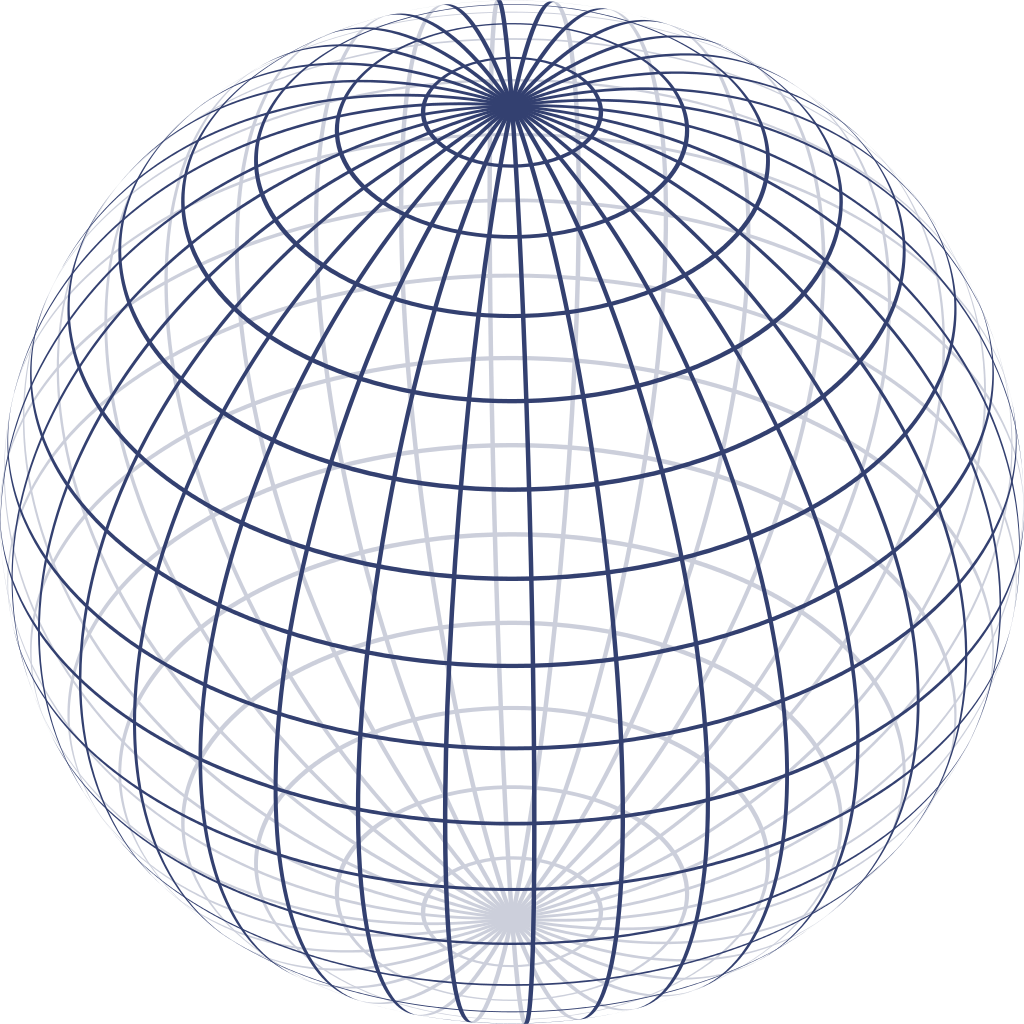
\includegraphics[width=3in]{./imagens/esfera}
\caption{Esfera}
\end{figure}


\section{Espaços Hiperbólicos}

\begin{defi}
	O \emph{espaço hiperbólico $n$-dimensional} é o conjunto
	\begin{equation*}
	\Hip^n \coloneqq \{x \in \R^{n+1}: x_1^2-x_2^2-\cdots -x_{n+1}^2=1,\\ x_0>0 \}.
	\end{equation*}
\end{defi}

\section{Toros}

\begin{defi}
	O \emph{toro $n$-dimensional} é o conjunto
	\begin{equation*}
	\T^n \coloneqq \R^n / \Z^n.
	\end{equation*}
\end{defi}

\begin{figure}[!h]
\centering
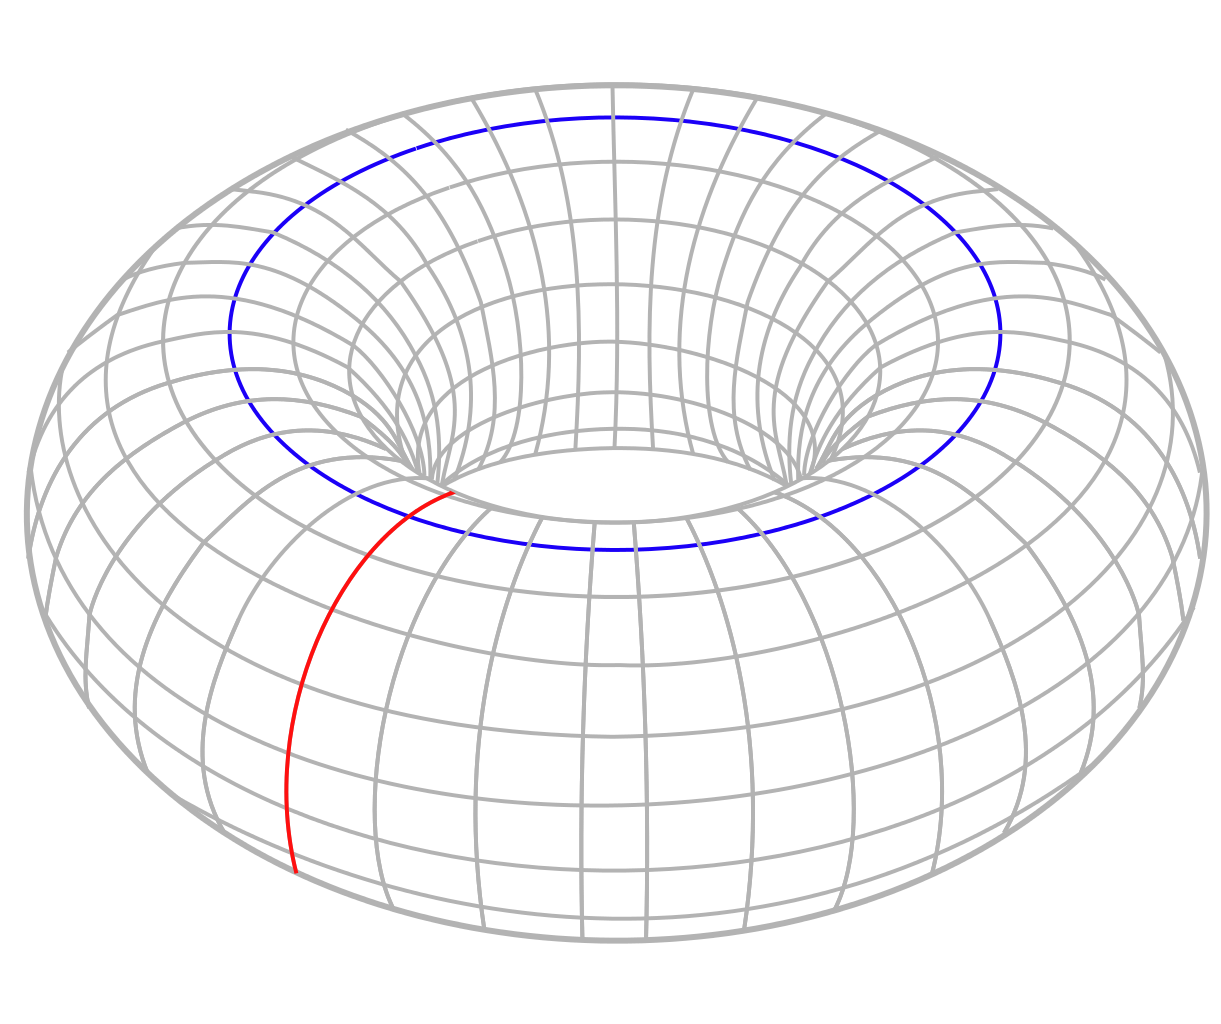
\includegraphics[width=3in]{./imagens/toro}
\caption{Toro}
\end{figure}


\chapter{Topologia dos Espaços Métricos}

\section{Métrica e Espaços Métricos}

\begin{defi}
	Seja $M$ um conjunto não vazio. Uma \emph{métrica} em $M$ é uma função $d: M \times M \to \R$ que satisfaz
	\begin{enumerate}
	\item Identidade dos Indescerníveis (Positiva Definida)\\
	$\forall p_1,p_2 \in M \qquad d(p_1,p_2)=0 \Leftrightarrow p_1=p_2$;
	\item Simetria \\
	$\forall p_1,p_2 \in M \qquad d(p_1,p_2)=d(p_2,p_1)$;
	\item Desigualdade Triangular \\
	$\forall p_1,p_2,p_3 \in M \qquad d(p_1,p_3) \leq d(p_1,p_2) + d(p_2,p_3)$.
	\end{enumerate}
	A \emph{distância} entre $p_1$ e $p_1$ é $d(p_1,p_2)$, a imagem de $(p_1,p_2)$ sob $d$.
\end{defi}

\begin{prop}
	Sejam $M$ um conjunto não vazio e $d$ uma métrica em $M$. Então
	\begin{enumerate}
	\item Não Negatividade \\
	$\forall p_1,p_2 \in M \qquad d(p_1,p_2) \geq 0$.
	\item Subaditividade Generalizada \\
	$\forall n \in \N^* \ \forall p_1,\ldots,p_n \in M \qquad d(p_1,p_n) \leq \displaystyle\sum_{i=1}^{n-1} d(p_i,p_{i+1})$.
%	\item Desigualdade Trianguar Alternativa \\
%	$\forall p_1,p_2,p_3 \in M \qquad |d(p_1,p_3)-d(p_2,p_3)| \leq d(p_1,p_2)$.
	\end{enumerate}
\end{prop}
\begin{proof}
	\begin{enumerate}
	\item Sejam $p_1,p_2 \in M$. Da desigualdade triangular e da simetria de $d$, segue que
	\begin{equation*}
	d(p_1,p_1) \leq d (p_1,p_2)+d(p_2,p_1)= 2 d(p_1,p_2),
	\end{equation*}
Mas $d(p_1,_1) = 0$, o que implica $d(p_1,p_1) \geq 0$.
	\item Para $n=1$, seja $p_1 \in M$; então $d(p_1,p_1)=0$ e $\sum_{i=1}^{0} d(p_i,p_{i+1})=0$, pois a soma é vazia. Para $n=2$, sejam $p_1,p_2 \in M$; então $d(p_1,p_2)$ e $\sum_{i=1}^{1} d(p_i,p_{i+1})=d(p_1,p_2)$, e vale a propriedade. Para $n=3$, sejam $p_1,p_2,p_3 \in M$; então a propriedade é a desigualdade triangulal. Agora, sejam $n \geq 4$, $p_1,\ldots,p_n \in M$ e assumamos que a propriedade vale para todo $k \in \N$, tal que $3 \leq k \leq n-1$. Então
	\begin{equation*}
	d(p_1,p_n) \leq \sum_{i=1}^{n-3} d(p_i,p_{i+1})+d(p_{n-2},p_n),
	\end{equation*}
pois essa soma tem $n-1$ termos e vale a hipótese de indução. Pela desigualdade triangular, vale que $d(p_{n-2},p_n) \leq d(p_{n-2},p_{n-1})+d(p_{n-1},p_n)$, e, portanto,
	\begin{align*}
	d(p_1,p_n) &\leq \sum_{i=1}^{n-3} d(p_i,p_{i+1})+d(p_{n-2},p_n)\\
			&\leq \sum_{i=1}^{n-3} d(p_i,p_{i+1}) + d(p_{n-2},p_{n-1})+d(p_{n-1},p_n) \\
			&= \sum_{i=1}^{n-1} d(p_i,p_{i+1}).
	\end{align*}
	\end{enumerate}
\end{proof}

\begin{prop}
	Sejam $M$ um conjunto não vazio e $(d_i)_{i \in \inte_n}$ métricas em $M$. Então a função
	\begin{align*}
	d: M \times M &\to \R \\
	 (p_1,p_2) &\mapsto \sum_{i=1}^n d_i(p_1,p_2)
	\end{align*}
é uma métrica em $M$.
\end{prop}
\begin{proof}
	\begin{enumerate}
	\item (Identidade dos Indiscerníveis) Sejam $p_1,p_2 \in M$. Suponhamos que
	\begin{equation*}
	d(p_1,p_2) = \sum_{i=1}^n d_i(p_1,p_2) = 0.
	\end{equation*}
Como, para todo $i \in \inte_n$, $d_i(p_1,p_2) \geq 0$, então, para todo $i \in \inte_n$, $d_i(p_1,p_2) = 0$. Logo $p_1=p_2$. Reciprocamente, suponhamos $p_1=p_2$. Então, para todo $i \in \inte_n$, $d_i(p_1,p_2)=0$, o que implica
	\begin{equation*}
	d(p_1,p_2) = \sum_{i=1}^n 0 = 0.
	\end{equation*}
	
	\item (Simetria) Sejam $p_1,p_2 \in M$. Então, pela simetria de $d_i$ para todo $i \in \inte_n$,
	\begin{equation*}
	d(p_1,p_2) = \sum_{i=1}^n d_i(p_1,p_2) = \sum_{i=1}^n d_i(p_2,p_1) = d(p_2,p_1).
	\end{equation*}
	
	\item (Desigualdade Triangular) Sejam $p_1,p_2,p_3 \in M$. Então, para todo $i \in \inte_n$, vale $d_i(p_1,p_3) \leq d_i(p_1,p_2)+d_i(p_2,p_3)$ pela desigualdade triangular de $d_i$, e segue que
	\begin{align*}
	d(p_1,p_3) &= \sum_{i=1}^n d_i(p_1,p_3) \\
				&\leq \sum_{i=1}^n (d_i(p_1,p_2)+d_i(p_2,p_3)) \\
				&= \sum_{i=1}^n d_i(p_1,p_2) + \sum_{i=1}^n d_i(p_2,p_3) \\
				&= d(p_1,p_2)+d(p_2,p_3).
	\end{align*}
	\end{enumerate}
\end{proof}

\begin{prop}
	Sejam $M$ um conjunto não vazio e $d_1,d_2$ métricas em $M$. Então a função
	\begin{align*}
	d: M \times M &\to \R \\
	 (p_1,p_2) &\mapsto \max\{d_1(p_1,p_2),d_2(p_1,p_2)\}
	\end{align*}
é uma métrica em $M$.
\end{prop}
\begin{proof}
	\begin{enumerate}
	\item (Identidade dos Indiscerníveis) Sejam $p_1,p_2 \in M$. Suponhamos que
	\begin{equation*}
	d(p_1,p_2)=\max\{d_1(p_1,p_2),d_2(p_1,p_2)\}=0.
	\end{equation*}
Então $d_1(p_1,p_2)=0$ ou $d_2(p_1,p_2)=0$. Em ambos os casos, temos $p_1=p_2$. Reciprocamente, suponhamos que $p_1=p_2$. Então $d_1(p_1,p_2)=0$ e $d_2(p_1,p_2)=0$, o que implica $d(p_1,p_2)=\max\{d_1(p_1,p_2),d_2(p_1,p_2)\}=0$.
	
	\item (Simetria) Sejam $p_1,p_2 \in M$. Então
	\begin{equation*}
	d(p_1,p_2) = \max\{d_1(p_1,p_2),d_2(p_1,p_2)\} = \max\{d_1(p_2,p_1),d_2(p_2,p_1)\} = d(p_2,p_1).
	\end{equation*}
	
	\item (Desigualdade Triangular) Sejam $p_1,p_2,p_3 \in M$. Então $d(p_1,p_3)=d_1(p_1,p_3)$ ou $d(p_1,p_3)=d_2(p_1,p_3)$. No primeiro caso, segue que
	\begin{equation*}
	d(p_1,p_3) = d_1(p_1,p_3) \leq d_1(p_1,p_2) + d_1(p_2,p_3) \leq d(p_1,p_2) + d(p_2,p_3).
	\end{equation*}
	No segudo caso, segue que
	\begin{equation*}
	d(p_1,p_3) = d_2(p_1,p_3) \leq d_2(p_1,p_2) + d_2(p_2,p_3) \leq d(p_1,p_2) + d(p_2,p_3).
	\end{equation*}
	\end{enumerate}
\end{proof}

\begin{defi}
	Um \emph{espaço métrico} é um par $(M,d)$, em que $M$ é um conjunto não vazio e $d$ é uma métrica em $M$. Os elementos de $M$ são \emph{pontos}.
\end{defi}



\section{Diâmetro, Bolas Abertas e Bolas Fechadas}

\begin{defi}
	Sejam $(M,d)$ um espaço métrico e $C \subseteq M$ um conjunto não vazio. O \emph{diâmetro} de $C$ é o número
	\begin{equation*}
	\diam(C) \coloneqq \sup (d(C \times C))
	\end{equation*}
se $d(C \times C) = \{d(p_1,p_2) : p_1,p_2 \in C\}$ é limitado superiormente, e $\infty$, caso contrário. Um \emph{conjunto limitado em $\bm M$} é um conjunto $C \subseteq M$ tal que $\diam(C) \in \R$. Uma \emph{sequência limitada em $\bm M$} é uma sequência $(p_n)_{n \in N}$ de pontos em $M$ tal que $\{p_n : n \in \N\}$ é limitado.
\end{defi}

\begin{defi}
	Sejam $(M,d)$ um espaço métrico, $c \in M$ e $r \in \R$ tal que $r>0$. A \emph{bola aberta} de centro $c$ e raio $r$ em $M$ é o conjunto
	\begin{equation*}
	\mathcal B_{r}(c) \coloneqq \{p \in M : d(c,p) < r\}.
	\end{equation*}
A \emph{bola fechada} de centro $c$ e raio $r$ em $M$ é o conjunto
	\begin{equation*}
	\overline {\mathcal B}_r(c) \coloneqq \{p \in M : d(c,p) \leq r\}.
	\end{equation*}
\end{defi}

\begin{prop}
	Seja $\bm M = (M,d)$ um espaço métrico e $C \subseteq M$ um conjunto. Então $C$ é um conjunto limitado se, e somente se, existem $r \in \R$ e $p \in M$ tais que $C \subseteq \mathcal B_r(p)$.
\end{prop}
\begin{proof}

\end{proof}



\section{Limites e Convergência de Sequências}

\begin{defi}
	Sejam $\bm M = (M,d)$ um espaço métrico, $(p_n)_{n \in \N}$ uma sequência de pontos em $M$ e $p \in M$. A sequência $(p_n)_{n \in \N}$  \emph{converge para o ponto $p$} se, para todo número real $\varepsilon > 0$, existe um número natural $N$ tal que
	\begin{equation*}
	\forall n \in \N \qquad n \geq N \Rightarrow p_n \in \mathcal B_\varepsilon(p).
	\end{equation*}
O ponto $p$ é um \emph{limite} da sequência e denota-se $(p_n) \conv p$. Caso contrário, a sequência não converge para $p$. Uma \emph{sequência convergente} é uma sequência que tem limite. Uma sequência \emph{divergente} é uma sequência que não tem limite.
\end{defi}

\begin{prop}
	Sejam $\bm M = (M,d)$ um espaço métrico e $p_1,p_2 \in M$ tais que $p_1 \neq p_2$. Se $r$ é um número real tal que $0 < r \leq  \frac{1}{2}  d(p_1,p_2)$, então $\mathcal B_r(p) \cap \mathcal B_r(p') = \emptyset$.
\end{prop}
\begin{proof}
	Se $p_1 \neq p_2$, então $d(p_1,p_2) > 0$. Portanto existe $r \in \R$ tal que $0 < r \leq \frac{1}{2} d(p_1,p_2)$. Suponhamos que existe $p \in \mathcal B_r(p) \cap \mathcal B_r(p')$. Então $d(p_1,p)<r$ e $d(p_2,p)<r$. Mas, pela desigualdade triangular, segue que
	\begin{equation*}
	d(p_1,p_2) \leq d(p_1,p) + d(p,p_2) < r + r \leq d(p_1,p_2),
	\end{equation*}
o que é absurdo. Portanto $\mathcal B_r(p) \cap \mathcal B_r(p') = \emptyset$.
\end{proof}

\begin{prop}
	Sejam $\bm M = (M,d)$ um espaço métrico e $(p_n)_{n \in \N}$ uma sequência de pontos em $M$. Se $(p_n)_{n \in \N}$ é convergente, então seu limite é único.
\end{prop}
\begin{proof}
	Suponhamos que $p,p'$ são limites de $(p_n)_{n \in \N}$. Se $p \neq p'$, então $d(p,p')>0$. Seja $\varepsilon \in \R$ tal que $0 < \varepsilon \leq \frac{1}{2} d(p,p')$. Então existe $N_1 \in \N$ tal que, para todo $n \in \N$, se $n \geq N_1$, então $p_n \in \mathcal B_\varepsilon(p)$, e existe $N_2 \in \N$ tal que, para todo $n \in \N$, se $n \geq N_2$, então $p_n \in \mathcal B_\varepsilon(p')$. Assim, definindo $N \coloneqq \max \{N_1,N_2\}$, segue que, se $n \geq N$, então $n \geq N_1$ e $n \geq N_2$, e, portanto, que $p_n \in \mathcal B_\varepsilon(p)$ e $p_n \in \mathcal B_\varepsilon(p')$; ou seja, $p_n \in \mathcal B_\varepsilon(p) \cap \mathcal B_\varepsilon(p')$, mas isso é absurdo, pois $\mathcal B_\varepsilon(p) \cap \mathcal B_\varepsilon(p')=\emptyset$. Portanto $p=p'$.
\end{proof}

	Essa proposição nos permite tratar o limite de uma sequência como um número único e, por isso, podemos usar a notação $\lim p_n = p$ para quando $(p_n) \conv p$.

\begin{prop}
	Sejam $\bm M = (M,d)$ um espaço métrico e $(p_n)_{n \in \N}$ uma sequência de pontos em $M$. Então $(p_n)_{n \in \N}$ é convergente se, e somente se, toda subsequência de $(p_n)_{n \in \N}$ é convergente.
\end{prop}
\begin{proof}
	Suponhamos que $(p_n) \conv p$ e seja $(p_{n_k})_{k \in \N}$ uma subsequência de $(p_n)_{n \in \N}$. Seja $\varepsilon \in \R$ tal que $\varepsilon > 0$. Como $(p_n) \conv p$, existe $N \in \N$ tal que, para todo $n \in \N$, se $n \geq N$, então $p_n \in \mathcal B_\varepsilon(p)$; como $(n_k)_{k \in \N}$ é estritamente crescente, existe $K \in \N$ tal que, para todo $k \in \N$, se $k \geq K$, então $n_k \geq N$. Mas então
	\begin{equation*}
	k \geq K \Rightarrow n_k \geq N \Rightarrow p_{n_k} \in \mathcal B_\varepsilon(p)
	\end{equation*}
e, portanto, $(p_{n_k}) \to p$.	Reciprocamente, se toda subsequência de $(p_n)_{n \in \N}$ converge para $p$, $(p_n)_{n \in \N}$, em particular, é uma dessas subsequências e, portanto, $(p_n) \conv p$.
\end{proof}

\begin{prop}
	Seja $\bm M = (M,d)$ um espaço métrico. Se uma sequência é convergente, então ela é limitada.
\end{prop}
\begin{proof}
	Seja $(p_n)_{n \in \N}$ uma sequência de pontos em $M$ tal que $(p_n) \conv p$. Então, para $\varepsilon = 1$, existe $N \in \N$ tal que, para todo $n \in \N$, se $n \geq N$, então $p_n \in \mathcal B_1(p)$. Assim, seja $l \in \R$ tal que
	\begin{equation*}
	l > \max(\{1\} \cup \{d(p,p_n) : n \in \inte_N\}),
	\end{equation*}
seque que, para todo $n \in \N$, $p_n \in \mathcal B_l(p)$ pois, se $0 \leq n \leq N$, $d(p,p_n) < l$ pela definição de $l$ e, se $n \geq N$, então $p_n \in \mathcal B_1(p) \subseteq B_l(p)$, pois $1 < l$. Logo $(p_n)_{n \in \N}$ é limitada.
\end{proof}

\begin{prop}
	Sejam $\bm M = (M,d)$ um espaço métrico, $C \subseteq M$ um conjunto e $p \in M$. Então existe uma sequência de pontos em $C$ que converge para $p$ se, e somente se, para todo número real $\varepsilon > 0$, $C \cap \mathcal B_\varepsilon(p) \neq \emptyset$.
\end{prop}
\begin{proof}
	Suponhamos que exista uma sequência $(p_n)_{n \in \N}$ de pontos em $C$ tal que $(p_n) \conv p$. Então, para todo número real $\varepsilon > 0$, existe $N \in \N$ tal que, para todo $n \in \N$, se $n \geq N$, então $p_n \in \mathcal B_\varepsilon(p)$. Mas isso implica que $p_n \in C \cap \mathcal B_\varepsilon(p)$. Reciprocamente, suponhamos que, para todo número real $\varepsilon > 0$, $C \cap \mathcal B_\varepsilon(p) \neq \emptyset$. Então, em particular, para todo $n \in \N$, escolhamos $p_n \in C \cap \mathcal B_{\frac{1}{n}}(p)$. Assim, temos a sequência $(p_n)_{n \in \N}$. Para mostrar que $(p_n) \conv p$, seja $\varepsilon \in \R$ tal que $\varepsilon > 0$. Então existe $N \in \N$ tal que $\frac{1}{N} \leq \varepsilon$. Mas isso implica que, para todo número natural $n \geq N$, $\frac{1}{n} \leq \frac{1}{N}$, e segue que
	\begin{equation*}
	d(p,p_n) < \frac{1}{n} \leq \frac{1}{N} \leq \varepsilon
	\end{equation*}
e, portanto, $(p_n) \conv p$.
\end{proof}

\begin{prop}
	Sejam $\bm M = (M,d)$ um espaço métrico, $p,q \in M$ e $(p_n)_{n \in \N}$ e $(q_n)_{n \in \N}$ sequências em $M$ que convergem para $p$ e $q$ respectivamente. Então a sequência $(d(p_n,q_n))_{n \in \N}$ em $\R$ converge para $d(p,q)$.
\end{prop}
\begin{proof}
	Para todo $n \in \N$, segue da desigualdade triangular que
	\begin{equation*}
	d(p_n,q_n) \leq d(p_n,p) + d(p,q) + d(q,q_n).
	\end{equation*}
Seja $\varepsilon > 0$ um número real. Então existem $N_1,_2 \in \N$ tais que
	\begin{equation*}
	\forall n \in \N \qquad n \geq N_1 \Rightarrow d(p,p_n) < \frac{\varepsilon}{2}
	\end{equation*}
e
	\begin{equation*}
	\forall n \in \N \qquad n \geq N_2 \Rightarrow d(q,q_n) < \frac{\varepsilon}{2}.
	\end{equation*}
Fazendo $N_3 \coloneqq \max\{N_1,N_2\}$, segue que
	\begin{equation*}
	\forall n \in \N \qquad n \geq N_3 \Rightarrow d(p_n,q_n) \leq d(p_n,p) + d(p,q) + d(q,q_n) < d(p,q) + \varepsilon;
	\end{equation*}
ou seja, $d(p_n,q_n) - d(p,q) < \varepsilon$. Analogamente, achamos $N_6 \in \N$ tal que
	\begin{equation*}
	\forall n \in \N \qquad n \geq N_3 \Rightarrow d(p_n,q_n) \leq d(p_n,p) + d(p,q) + d(q,q_n) < d(p,q) + \varepsilon
	\end{equation*}
e fazendo $n \coloneqq \max\{N_3,N_6\}$, segue que
	\begin{equation*}
	\forall n \in \N \qquad n \geq N \Rightarrow |d(p,q) - d(p_n,q_n)| < \varepsilon,
	\end{equation*}
o que mostra que $(d(p_n,q_n)) \conv d(p,q)$ em $\R$.
	
\end{proof}


\section{Sequências de Cauchy}

\begin{defi}
	Seja $\bm M = (M,d)$ um espaço métrico. Uma \emph{sequência de Cauchy em $\bm M$} é uma sequência $(p_n)_{n \in \N}$ de pontos em $M$ tal que, para todo número real $\varepsilon > 0$, existe um número natural $N$ satisfazendo
	\begin{equation*}
	\forall n,m \in \N \qquad n,m \geq N \Rightarrow d(p_n,p_m) < \varepsilon.
	\end{equation*}
\end{defi}

\begin{prop}
	Sejam $\bm M = (M,d)$ um espaço métrico e $(p_n)_{n \in \N}$ uma sequência convergente em $M$. Então $(p_n)_{n \in \N}$ é uma sequência de Cauchy.
\end{prop}
\begin{proof}
	Seja $(p_n)_{n \in \N}$ uma sequência em $M$ que converge para $p$. Seja $\varepsilon \in \R$ tal que $\varepsilon > 0$. Então $\frac{1}{2}\varepsilon > 0$ é um número real e segue que existe $N \in \N$ tal que, para todo número natural $n \geq N$, $p_n \in \mathcal B_{\frac{1}{2}\varepsilon}(p)$. Assim, segue que	
	\begin{equation*}
	\forall n,m \in \N \qquad n,m \geq N \Rightarrow d(p_n,p_m) \leq d(p_n,p) + d(p,p_m) < \frac{\varepsilon}{2} + \frac{\varepsilon}{2} = \varepsilon,
	\end{equation*}
o que mostra que $(p_n)_{n \in \N}$ é uma sequência de Cauchy.
\end{proof}

\begin{prop}
	Sejam $\bm M = (M,d)$ um espaço métrico e $(p_n)_{n \in \N}$ uma sequência de Cauchy em $\bm M$. Se existe uma subsequência $(p_{n_k})_{k \in \N}$ de $(p_n)_{n \in \N}$ que é convergente, então $(p_n)_{n \in \N}$ é convergente.
\end{prop}
\begin{proof}
	Seja $(p_{n_k})_{k \in \N}$ uma subsequência de $(p_n)_{n \in \N}$ que converge  para $p$. Seja $\varepsilon > 0$ um número real. Como $(p_n)_{n \in \N}$ é uma sequência de Cauchy e $\frac{1}{2}\varepsilon > 0$ é um número real, existe um número natural $N$ tal que
	\begin{equation*}
	\forall n,m \in \N \qquad n,m \geq N \Rightarrow d(p_n,p_m) < \frac{\varepsilon}{2}.
	\end{equation*}
Como $(p_{n_k})_{k \in \N}$ é uma subsequência convergente, existe $K_1 \in \N$ tal que
	\begin{equation*}
	\forall k \in \N \qquad k \geq K_1 \Rightarrow d(p,p_{n_k}) < \frac{\varepsilon}{2}.
	\end{equation*}
Como $(n_k)_{k \in \N}$ é uma sequência estritamente crescente, existe $K_2 \in \N$ tal que, para todo número natural $k \geq K_2$, $n_k \geq N$. Assim, tomando $K \coloneqq \max\{K_1,K_2\}$, segue que, para todo número natural $n \in \N$, existe $k \in \N$ tal que $n_k \geq N$ e,  pela desigualdade triangular, que
	\begin{equation*}
	\forall n \in \N \qquad n \geq N \Rightarrow d(p_n,p) \leq d(p_n,p_{n_k}) + d(p_{n_k},p) < \frac{\varepsilon}{2}+\frac{\varepsilon}{2}=\varepsilon.
	\end{equation*}
\end{proof}

\begin{prop}
	Sejam $\bm M = (M,d)$ um espaço métrico e $(p_n)_{n \in \N}$ uma sequência de Cauchy em $\bm M$. Então $(p_n)_{n \in \N}$ é limitada em $\bm M$.
\end{prop}
\begin{proof}
	Como $(p_n)_{n \in \N}$ é uma sequência de Cauchy em $\bm M$, para $\varepsilon=1$, existe $N \in \N$ tal que
	\begin{equation*}
	\forall n,m \in \N \qquad n,m \geq N \Rightarrow d(p_n,p_m)<1.
	\end{equation*}
	Definamos $P \coloneqq \{p_n : n \in \N\}$. Então segue que
	\begin{equation*}
	\diam(P) = \sup \{d(p_n,p_m) : n,m \in \N\} = \max\{1 \cup \{d(p_n,p_m) : 0 \leq n,m \leq N\}\} \in \R,
	\end{equation*}
o que mostra que $(p_n)_{n \in \N}$ é limitada.
\end{proof}

\section{Interior e Conjuntos Abertos}

\begin{defi}
	Sejam $\bm M = (M,d)$ um espaço métrico e $C \subseteq M$ um conjunto. Um \emph{ponto interior} de $C$ é um ponto $p \in C$ para o qual existe um número real $r > 0$ tal que $\mathcal B_r(p) \subseteq C$. O \emph{interior} de $C$ é o conjunto $C^\circ$ de todos pontos interiores de $C$.
\end{defi}

%\mathring é um comando iteressante, mas não serve tão bem aos meus propósitos.

\begin{prop}
	Sejam $\bm M = (M,d)$ um espaço métrico e $A,B \subseteq M$ conjuntos. Então
	\begin{enumerate}
	\item $A^\circ \subseteq A$.
	\item $A^\circ \cup B^\circ \subseteq (A \cup B)^\circ$.
	\end{enumerate}
\end{prop}

Da definição, segue que $C^\circ \subseteq C$. A inclusão contrária caracteriza a próxima definição.

\begin{defi}
	Seja $\bm M = (M,d)$ um espaço métrico. Um \emph{conjunto aberto} de $\bm M$ é um conjunto $A \subseteq M$ tal que $A = A^\circ$. O conjunto dos conjuntos abertos de $\bm M$ é denotado $\mathcal T_{\bm M}$.
\end{defi}

\begin{prop}
	Seja $\bm M = (M,d)$ um espaço métrico. Então
	\begin{enumerate}
	\item Para todo $c \in M$ e para todo número real $r > 0$, a bola aberta $B_r(c)$ é um conjunto aberto;
	\item O conjunto $\mathcal T_{\bm M}$ é uma topologia de $M$.
		\begin{enumerate}
			\item $\emptyset,M \in \mathcal T_{\bm M}$;
			\item $(A_i)_{i \in I} \subseteq \mathcal T_{\bm M} \Rightarrow \displaystyle\bigcup_{i \in I} A_i \in \mathcal T_{\bm M}$;
			\item $(A_i)_{i \in \inte_n} \subseteq \mathcal T_{\bm M} \Rightarrow \displaystyle\bigcap_{i=1}^n A_i \in \mathcal T_{\bm M}$.
		\end{enumerate}
	\end{enumerate}
\end{prop}
\begin{proof}
	\begin{enumerate}
	\item Sejam $c \in M$ e $r \in \R_+^*$. Queremos mostrar que $\mathcal B_r(c)$ é aberto. Para isso, seja $p \in \mathcal B_r(c)$. Então segue que $d \coloneqq d(c,p) < r$, pela definição de bola aberta, e, portanto, $r-d \in \R_+^*$. Para mostrar que essa bola centrada em $p$ está contida na bola maior centrada em $c$, seja $p' \in \mathcal B_{r-d}(p)$. Então $d(p,p')<r-d$ e, pela desigualdade triangular, segue que
	\begin{equation*}
	d(c,p') \leq d(c,p) + d(p,p') < D + (r-d) = r,
	\end{equation*}
o que mostra que $p' \in \mathcal B_r(c)$ e que, portanto, $\mathcal B_s(p) \subseteq \mathcal B_r(c)$. Assim, mostramos que $\mathcal B_r(p)$ é aberta.
	
	\item
		\begin{enumerate}
		\item Podemos notar que $\emptyset$ é aberto por vacuidade, pois, se não fosse, existiria $p \in \emptyset$ para o qual não há $r \in \R_+^*$ satisfazendo $\mathcal B_r(p) \subseteq A$, o que é absurdo.
	Para mostrar que $M$ é aberto, sejam $p \in M$ e $r \in \R_+^*$. Então $\mathcal B_r(p) \subseteq M$, pois qualquer bola aberta é subconjunto de $M$. Portanto $M$ é aberto.
	
		\item Seja $(A_i)_{i \in I}$ uma família de abertos em $\bm M$ e seja $p \in (A_i)_{i \in I}$. Então existe $k \in I$ tal que $p \in A_k$. Como $A_k$ é aberto, então existe $r \in \R_+^*$ tal que $\mathcal B_r(p) \subseteq A_k$. Como $A_k \subseteq (A_i)_{i \in I}$, segue que $\mathcal B_r(p) \subseteq (A_i)_{i \in I}$ e que, portanto, $(A_i)_{i \in I}$ é aberto.
	
		\item Seja $(A_i)_{i \in \inte_n}$ uma sequência de abertos em $\bm M$ e seja $p \in (A_i)_{i \in \inte_n}$. Então, para todo $k \in \inte_n$, $p \in A_k$. Como, para todo $k \in \inte_n$, $A_k$ é aberto, segue que existe $r_k \in \R_+^*$ tal que $\mathcal B_{r_k}(p) \subseteq A_k$, Seja $r \coloneqq \min \{r_k : k \in \inte_n\}$. Então, para todo $k \in \inte_n$, vale $\mathcal B_r(p) \subseteq \mathcal B_{r_k}(p)$, e segue que $\mathcal B_r(p) \subseteq A_k$ e, portanto, $\mathcal B_r(p) \subseteq (A_i)_{i \in \inte_n}$, o que mostra que $(A_i)_{i \in \inte_n}$ é aberto.
		\end{enumerate}		
	\end{enumerate}
\end{proof}

\begin{prop}
	Sejam $\bm M = (M,d)$ um espaço métrico e $C \subseteq M$ um conjunto. Então o interior de $C$ é a união de todos os conjuntos abertos de $\bm M$ que são subconjuntos de $C$.
\end{prop}

\begin{prop}
	Sejam $\bm M = (M,d)$ um espaço métrico e $A,B \subseteq M$ conjuntos. Então
	\begin{enumerate}
	\item $C^\circ$ é um conjunto aberto.
	\item $\emptyset^\circ = \emptyset$.
	\item $M^\circ = M$.
	\item ...
	\end{enumerate}
\end{prop}

\section{Fecho e Conjuntos Fechados}

\begin{defi}
	Sejam $\bm M = (M,d)$ um espaço métrico e $C \subseteq M$ um conjunto. Um \emph{ponto aderente} a $C$ é um ponto $p \in M$ para o qual existe uma sequência $(p_n)_{n \in \N}$ de pontos de $C$ que converge para $p$. O \emph{fecho} de $C$ é o conjunto $\overline C$ de todos os pontos aderentes a $C$.
\end{defi}

\begin{prop}
	Sejam $\bm M = (M,d)$ um espaço métrico e $A,B \subseteq M$ conjuntos. Então
	\begin{enumerate}
	\item $\overline \emptyset = \emptyset$.
	\item $A \subseteq \overline A$.
	\item $\overline{(A \cup B)} = \overline A \cup \overline B$.
	\item $\overline{(\overline A)} = \overline A$.
	\end{enumerate}
\end{prop}

Da definição, segue que $C \subseteq \overline C$. A inclusão contrária caracteriza a próxima definição.

\begin{defi}
	Seja $\bm M = (M,d)$ um espaço métrico. Um \emph{conjunto fechado} de $\bm M$ é um conjunto $F \subseteq M$ tal que $F = \overline F$. O conjuntos dos conjuntos fechados de $\bm M$ é denotado $\complement( \mathcal T_{\bm M})$.
\end{defi}

\begin{prop}
	Sejam $\bm M = (M,d)$ um espaço métrico e $F \subseteq M$. Então $F$ é um conjunto fechado se, e somente se, $F^\complement$ é um conjunto aberto.
\end{prop}
\begin{proof}
	Suponhamos que $F$ é um conjunto fechado. Se $F^\complement = \emptyset$, Mas $\emptyset$ é aberto pois, caso contrário, existe $p \in \emptyset$ para o qual não há número real $\varepsilon > 0$ tal que $\mathcal B_\varepsilon(p) \subseteq \emptyset$, mas isso é absurdo. Se $F^\complement \neq \emptyset$, seja $p \in F^\complement$. Se não existe número real $\varepsilon > 0$ tal que $\mathcal B_\varepsilon(p) \subseteq F^\complement$, então, para todo número real $\varepsilon > 0$, $F \cap \mathcal B_\varepsilon(p) \neq \emptyset$. Mas isso implica que existe uma sequência $(p_n)_{n \in \N}$ de pontos em $F$ tal que $(p_n) \conv p$. Como $F$ é fechado, isso implica $p \in F$, o que é uma contradição. Então existe número real $\varepsilon > 0$ tal que $\mathcal B_\varepsilon(p) \subseteq F^\complement$, e isso mostra que $F^\complement$ é aberto.
	
	Reciprocamente, suponhamos que $F^\complement$ é aberto. Se $F = \emptyset$, então $F$ é fechado. Se $F \neq \emptyset$, seja $(p_n)_{n \in \N}$ uma sequência em $F$ que converge para $p \in M$. Suponhamos que $p \notin F$. Então $p \in F^\complement$ e, como $F^\complement$ é aberto, existe um número real $\varepsilon > 0$ tal que $\mathcal B_\varepsilon(p) \subseteq F^\complement$. Como $(p_n) \conv p$, existe $N \in \N$ tal que, para todo $n \in \N$, se $n \geq N$, então $p_n \in \mathcal B_\varepsilon(p)$. Mas isso implica que $p_{N} \in \mathcal B_\varepsilon(p) \subseteq F^\complement$, o que é absurdo, pois $p_n \in F$. Portanto $p \in F$ e isso mostra que $F$ é fechado.
\end{proof}

\begin{prop}
	Seja $\bm M = (M,d)$ um espaço métrico. Então
	\begin{enumerate}
	\item Para todo $c \in M$ e para todo número real $r > 0$, a bola fechada $\overline B_r(c)$ é um conjunto fechado;
	\item O conjunto $\complement(\mathcal T_{\bm M})$ satisfaz
		\begin{enumerate}
			\item $\emptyset,M \in \complement(\mathcal T_{\bm M})$;
			\item $(A_i)_{i \in I} \subseteq \complement(\mathcal T_{\bm M}) \Rightarrow \displaystyle\bigcap_{i \in I} A_i \in \complement(\mathcal T_{\bm M})$;
			\item $(A_i)_{i \in \inte_n} \subseteq \complement(\mathcal T_{\bm M}) \Rightarrow \displaystyle\bigcup_{i=1}^n A_i \in \complement(\mathcal T_{\bm M})$.
		\end{enumerate}
	\end{enumerate}
\end{prop}
\begin{proof}
	\begin{enumerate}
	\item ...
	
	\item Segue da proposição anterior e do fato de que $\mathcal T_{\bm M}$ é uma topologia de $\bm M$.
	\end{enumerate}
\end{proof}

\begin{prop}
	Sejam $\bm M = (M,d)$ um espaço métrico e $C \subseteq M$ um conjunto. Então o fecho de $C$ é a interseção de todos os conjuntos fechados de $\bm M$ dos quais $C$ é subconjunto.
\end{prop}

\begin{prop}
	Sejam $\bm M = (M,d)$ um espaço métrico e $A,B \subseteq M$ conjuntos. Então
	\begin{enumerate}
	\item $\overline A$ é um conjunto fechado.
	\item $\overline \emptyset = \emptyset$.
	\item $\overline M = M$.
	\item Se $A \subseteq B$, então $\overline A \subseteq \overline B$.
	\end{enumerate}
\end{prop}

\begin{prop}
	Sejam $\bm M = (M,d)$ um espaço métrico e $A \subseteq M$ conjuntos. Então
	\begin{enumerate}
	\item $(\overline A)^\complement = (A^\complement)^\circ$.
	\item $(A^\circ)^\complement = \overline{(A^\complement)}$.
	\end{enumerate}
\end{prop}

\section{Conjuntos Densos}

\begin{defi}
	Sejam $\bm M$ um espaço métrico e $C \subseteq M$ um conjunto. Um conjunto \emph{denso em $C$} é um conjunto $D \subseteq M$ tal que $C \subseteq \overline D$.
\end{defi}

	Isso que dizer que, para todo ponto de $C$, existe uma sequência em $D$ que converge para esse ponto.
	
\begin{prop}
	Sejam $\bm M = (M,d)$ um espaço métrico e $C,D \subseteq M$ conjuntos. Então $D$ é denso em $C$ se, e somente se, para todo conjunto aberto $A$ de $\bm M$, $A \cap C \neq \emptyset$ implica $A \cap D \neq \emptyset$.
\end{prop}
\begin{proof}
	Suponhamos que $D$ é denso em $C$. Sejam $A$ um conjunto aberto de $\bm M$ tal que $A \cap C \neq \emptyset$ e seja $p \in A \cap C$. Como $D$ é denso em $C$ e $p \in C$, existe uma sequência $(p_n)_{n \in \N}$ em $D$ que converge para $p$. Como $A$ é aberto e $p \in A$, existe um número real $\varepsilon>0$ tal que $\mathcal B_\varepsilon(p) \subseteq A$. Então, como $(p_n) \conv p$, existe um número natural $N$ tal que, para todo natural $n \geq N$, $p_n \in \mathcal B_\varepsilon(p)$. Mas isso implica que $p_n \in A \cap D$.
	
	Reciprocamente, suponhamos que, para todo conjunto aberto $A$ de $\bm M$, $A \cap C \neq \emptyset$ implica $A \cap D \neq \emptyset$. Se $C=\emptyset$, então $C \subseteq \overline D$. Se $C \neq \emptyset$, seja $p \in C$. Para todo $n \in \N$, o conjunto $\mathcal B_\frac{1}{n}(p)$ é um conjunto aberto que contém $p$. Mas então $\mathcal B_\frac{1}{n}(p) \cap C \neq \emptyset$, o que implica $\mathcal B_\frac{1}{n}(p) \cap D \neq \emptyset$. Para cada $n \in \N$, escolhamos $p_n \in B_\frac{1}{n}(p) \cap D$. Assim, temos uma sequência $(p_n)_{n \in \N}$ de pontos em $D$ que converge para $p$, pois, para todo número real $\varepsilon>0$, existe um natural $N$ tal que $\frac{1}{N} \leq \varepsilon$ e, então
	\begin{equation*}
	\forall n \in \N \qquad n \geq N \Rightarrow \frac{1}{n} \leq \frac{1}{N} \leq \varepsilon \Rightarrow p_n \in \mathcal B_\frac{1}{n}(p) \subseteq \mathcal B_\frac{1}{N}(p) \subseteq \mathcal B_\varepsilon(p).
	\end{equation*}
	Isso mostra que $p \in \overline D$ e, portanto, que $C \subseteq \overline D$.
\end{proof}

\begin{prop}
	Sejam $\bm M_1$ e $\bm M_2$ espaços métricos e $f,g: M_1 \to M_2$ funções contínuas. Então o conjunto 
	\begin{equation*}
	F \coloneqq \{p \in M_1 : f(p)=g(p)\}
	\end{equation*}
é um conjunto fechado.
\end{prop}
\begin{proof}
	Se $F=\emptyset$, então $F$ é fechado. Se $F \neq \emptyset$, seja $(p_n)_{n \in \N}$ uma sequência em $F$ que converge para $p \in M_1$. Mostraremos que $p \in F$. Como $f$ e $g$ são contínuas em $p$, segue que
	\begin{equation*}
	(f(p_n)) \conv f(p) \e (g(p_n)) \conv g(p).
	\end{equation*}
	Como $(p_n)_{n \in \N}$ é uma sequência em $F$, as sequências $(f(p_n))_{n \in \N}$ e $(g(p_n))_{n \in \N}$ são a mesma sequência e segue da unicidade do limite que $f(p)=g(p)$, o que mostra que $p \in F$ e que, portanto, $F$ é um conjunto fechado.
\end{proof}

\begin{prop}
	Sejam $\bm M_1$ e $\bm M_2$ espaços métricos, $f,g: M_1 \to M_2$ funções contínuas e $C,D \subseteq M_1$ conjuntos tais que $D$ é denso em $C$. Se $f|_D = g|_D$, então $f|_C = g|_C$.
\end{prop}
\begin{proof}
	Pela proposição anterior, sabemos que $F \coloneqq \{p \in M_1 : f(p)=g(p)\}$ é um conjunto fechado. Como $f|_D = g|_D$, então $D \subseteq F$. Mas isso significa que $\overline D \subseteq \overline F = F$ e, como $D$ é denso em $C$, segue que $C \subseteq \overline D \subseteq F$ e, portanto, que $f|_C = g|_C$. 
\end{proof}


\section{Continuidade}

\begin{defi}
	Sejam $\bm M_1 = (M_1,d_1)$ e $\bm M_2 = (M_2,d_2)$ espaços métricos, $f: M_1 \to M_2$ uma função e $p \in M$. A função $f$ é \emph{contínua em $p$} se, para todo número real $\varepsilon > 0$, existe um número real $\delta > 0$ tal que
%	\begin{equation*}
%	\forall x \in M_1 \qquad d_1(p,x) < \delta \Rightarrow d_2(f(p),f(x)) < \varepsilon.
%	\end{equation*}
	\begin{equation*}
	\forall x \in M_1 \qquad x \in \mathcal B_\delta(p) \Rightarrow f(x) \in \mathcal B_\varepsilon(f(p)).
	\end{equation*}
Caso contrário, a função $f$ não é contínua em $p$, ela é \emph{descontínua} em $p$.
\end{defi}

	Denotamos as bolas abertas em $\bm M_1$ e em $\bm M_2$ por $\mathcal B$, mas deve-se perceber que elas são relativas a métricas possivelmente diferentes. 

\begin{prop}
	Sejam $\bm M_1 = (M_1,d_1)$ e $\bm M_2 = (M_2,d_2)$ espaços métricos, $f: M_1 \to M_2$ uma função e $p \in M_1$. Então $f$ é contínua em $p$ se, e somente se, para toda sequência $(p_n)_{n \in \N}$ de pontos em $M_1$ que converge para $p$, a sequência $(f(p_n))_{n \in \N}$ de pontos em $M_2$ converge para $f(p)$; ou seja
	\begin{equation*}
	\lim f(p_n) = f(\lim p_n).
	\end{equation*}
\end{prop}
\begin{proof}
	Suponhamos que $f$ é contínua em $p$. Seja $(p_n)_{n \in \N}$ uma sequência de pontos em $M_1$ que converge para $p$. Seja um número real $\varepsilon > 0$. Como $f$ é contínua, existe um número real $\delta > 0$ tal que $p_n \in \mathcal B_\delta(p)$ implica $f(p_n) \in \mathcal B_\varepsilon(f(p))$. Mas, como $(p_n) \conv p$, existe $N \in \N$ tal que
	\begin{equation*}
	\forall n \in \N \qquad n \geq N \Rightarrow p_n \in \mathcal B_\delta(p) \Rightarrow f(p_n) \in \mathcal B_\varepsilon(f(p))
	\end{equation*}
o que mostra que $(f(p_n)) \conv f(p)$.
	
	Reciprocamente, suponhamos que, para toda sequência $(p_n)_{n \in \N}$ em $M_1$ que converge para $p$, a sequência $(f(p_n))_{n \in \N}$ converge para $f(p)$. Suponhamos, por absurdo, que $f$ não é contínua em $p$. Então existe um número real $\varepsilon > 0$ tal que, para todo número real $\delta > 0$, existe $x \in M_1$ tal que $x \in \mathcal B_\delta(p)$, mas $f(x) \notin \mathcal B_\varepsilon(f(p))$. Vamos mostrar que isso implica que existe uma sequência $(p_n)_{n \in \N}$ em $M_1$ que converge para $p$, mas que a sequência $(f(p_n))_{n \in \N}$ não converge para $f(p)$; ou seja, que existe um número real $\varepsilon > 0$ tal que, para todo número natural $N$, existe $n \in \N$ tal que $n \geq N$, mas $f(p_n) \notin \mathcal B_\varepsilon(f(p))$. Seja $n \in \N$ e tomemos $\delta = \frac{1}{n}$. Então existe $x \in M_1$ tal que $x \in \mathcal B_\frac{1}{n}(p)$, mas $f(x) \notin \mathcal B_\varepsilon(f(p))$. Nomeando esse $x \in M_1$ de $p_n$, obtemos uma sequência $(p_n)_{n \in \N}$ que converge para $p$ pois, para todo número real $\varepsilon' > 0$, existe um número natural $N \in \N$ tal que $\frac{1}{N} \leq \varepsilon'$ e isso implica que
\begin{equation*}
	\forall n \in \N \qquad n \geq N \Rightarrow \frac{1}{n} \leq \frac{1}{N} \leq \varepsilon' \Rightarrow p_n \in \mathcal B_\frac{1}{n}(p) \subseteq \mathcal B_\frac{1}{N}(p) \subseteq \mathcal B_{\varepsilon'}(p).
	\end{equation*}
	No entanto, $(f(p_n))_{n \in \N}$ é uma sequência que não converge para $f(p)$ pois, considerando o $\varepsilon$ original tomado da descontinuidade de $f$, para todo número natural $N$, $f(p_N) \notin \mathcal B_\varepsilon(f(p))$ e isso contradiz a hipótese de que, para toda sequência $(p_n)_{n \in \N}$ em $M_1$ que converge para $p$, a sequência $(f(p_n))_{n \in \N}$ converge para $f(p)$. Portanto $f$ é contínua.	
\end{proof}

\begin{defi}
	Sejam $\bm M_1 = (M_1,d_1)$ e $\bm M_2 = (M_2,d_2)$ espaços métricos, $D \subseteq M_1$ e $f: D \to M_2$ uma função. A função $f$ é contínua em $D$ se ela é contínua em todo ponto de $D$ e é \emph{contínua} de $D = M_1$. Caso contrário, a função $f$ é \emph{descontínua} em $D$. Para $D=M_1$, dizemos que $f$ é contínua ou descontínua.
\end{defi}

\begin{prop}
	Para funções contínuas, imagem inversa de aberto é aberto.
\end{prop}



\section{Continuidade Uniforme}

\begin{defi}
	Sejam $\bm M_1 = (M_1,d_1)$ e $\bm M_2 = (M_2,d_2)$ espaços métricos. Uma função \emph{uniformemente contínua} é uma função $f: M_1 \to M_2$ tal que, para todo número real $\varepsilon > 0$, existe um número real $\delta > 0$ tal que
	\begin{equation*}
	\forall p_1,p_2 \in M_1 \qquad d_1(p_1,p_2) < \delta \Rightarrow d_2(f(p_1),f(p_2)) < \varepsilon.
	\end{equation*}
\end{defi}

\begin{prop}
	Sejam $\bm M_1 = (M_1,d_1)$ e $\bm M_2 = (M_2,d_2)$ espaços métricos, $f: M_1 \to M_2$ uma função uniformemente contínua e $(p_n)_{n \in \N}$ uma sequência em $M_1$. Então, se $(p_n)_{n \in \N}$ é uma sequência de Cauchy, a sequência $(f(p_n))_{n \in \N}$ em $M_2$ é uma sequência de Cauchy.
\end{prop}
\begin{proof}
	Seja $(p_n)_{n \in \N}$ é uma sequência de Cauchy. Seja $\varepsilon > 0$ um número real. Da continuidade uniforme de $f$, existe um número real $\delta > 0$ tal que, para todo $p,p' \in M_1$, $d_1(p,p') < \delta$ implica $d_2(f(p),f(p')) < \varepsilon$. Como $(p_n)_{n \in \N}$ é sequência de Cauchy, existe $N \in \N$ tal que
	\begin{equation*}
	\forall n,m \in \N \qquad n,m \geq N \Rightarrow d_1(p_n,p_m) < \delta.
	\end{equation*}
Mas, da continuidade uniforme de $f$, isso implica que
	\begin{equation*}
	\forall n,m \in \N \qquad n,m \geq N \Rightarrow d_1(p_n,p_m) < \delta  \Rightarrow d_2(f(p_n),f(p_m)) < \varepsilon,
	\end{equation*}
e isso mostra que $(f(p_n))_{n \in \N}$ é uma sequênca de Cauchy.
\end{proof}


\section{Espaços Métricos Completos}

\begin{defi}
	Seja $\bm M$ um espaço métrico. Um conjunto \emph{completo} em $\bm M$ é um conjunto $C \subseteq M$ em que toda sequência de Cauchy em $\bm M$ converge para um ponto em $C$. Um espaço métrico \emph{completo} é um espaço métrico  $\bm M$ em que $M$ é um conjunto completo.
\end{defi}

\begin{prop}
	Seja $\bm M = (M,d)$ um espaço métrico e $C \subseteq M$ um conjunto. Se $C$ é completo, então $C$ é fechado.
\end{prop}
\begin{proof}
	Seja $(p_n)_{n \in \N}$ uma sequêcia em $C$. Então $(p_n)_{n \in \N}$ é uma sequência de Cauchy e, como $C$ é completo, $(p_n)_{n \in \N}$ converge para um ponto em $C$. Mas isso significa que $C$ é fechado.
\end{proof}

\begin{prop}
	Seja $\bm M = (M,d)$ um espaço métrico, $C,F \subseteq M$ conjuntos tais que $F \subseteq C$. Se $C$ é completo e $F$ é fechado, então $F$ é completo.
\end{prop}
\begin{proof}
	Seja $(p_n)_{n \in \N}$ uma sequêcia de Cauchy em $F$. Então $(p_n)_{n \in \N}$ é uma sequência de Cauchy em $C$ e, como $C$ é completo, $(p_n)_{n \in \N}$ converge. Porém, como $F$ é fechado, então $(p_n)_{n \in \N}$ converge para um ponto em $F$, o que mostra que $F$ é completo.
\end{proof}

\begin{teo}
	Seja $\bm M =(M,d)$ um espaço métrico. Então $\bm M$ é completo se, e somente se, para toda sequência descrescente $(F_n)_{n \in \N}$ de conjuntos não vazios e fechados em $\bm M$ tais que $(\diam(F_n))_{n \in \N} \conv 0$ em $\R$, vale que
	\begin{equation*}
	\bigcap_{n \in \N} A_n \neq \emptyset.
	\end{equation*}
\end{teo}
\begin{proof}

\end{proof}

\subsection{Espaços Métricos Completos e Continuidade Uniforme}

\begin{teo}
	Sejam $\bm M_1 = (M_1,d_1)$  um espaço métrico, $\bm M_2 = (M_2,d_2)$ espaço métrico completo, $D \subseteq M_1$ um conjunto denso em $M_1$ e $f: D \to M_2$ uma função uniformemente contínua. Então $f$ tem uma única extensão para uma função uniformemente contínua $f^*: M_1 \to M_2$. Ainda, se $f$ é uma isometria, então $f^*$ é uma isometria.
\end{teo}
\begin{proof}
	Seja $p \in M_1$. Como $D$ é denso em $M_1$, existe uma sequência $(p_n)_{n \in \N}$ em $D$ que converge para $p$. Como $(p_n)_{n \in \N}$ é convergente, é uma sequência de Cauchy e, como $f$ é uniformemente contínua em $D$, segue que $(f(p_n))_{n \in \N}$ é uma sequência de Cauchy em $M_2$. Mas $M_2$ é completo, o que implica que $(f(p_n))_{n \in \N}$ converge para um ponto $p' \in M_2$. Definimos, portanto, a função $f^*$ em $p$ como $f^*(p)=p'$. Precisamos mostrar que $f^*$ independe da escolha da sequência em $D$ que converge para $p$. Se $(q_n)_{n \in \N}$ é uma sequência em $D$ que converge para $p$, definamos a sequência $(r_n)_{n \in \N}$ em $D$ por
	\begin{equation*}
	r_n \coloneqq
			\begin{cases}
			p_n &\text{se $n=2k$}\\
			q_n &\text{se $n=2k+1$}.
			\end{cases}
	\end{equation*}
A sequência $(r_n)_{n \in \N}$ converge para $p$ e, portanto, é uma sequência de Cauchy. A continuidade uniforme de $f$ implica que a sequência $(f(r_n))_{n \in \N}$ é de Cauchy e, portanto, como $(f(p_n))_{n \in \N}=(f(r_{2k}))_{k \in \N}$ é uma subsequência que converge para $p'$, a sequência $(f(r_n))_{n \in \N}$ converge para $p'$, o que implica que a subsequência $(f(q_n))_{n \in \N}=(f(r_{2k+1}))_{k \in \N}$ converge para $p'$. Assim, mostramos que $f^*$ está bem definida. Claramente, se $p \in D$, então $f(p)=f^*(p)$, pois, como $D$ é denso em $M_1$, se $(p_n)_{n \in \N}$ é uma sequência em $D$ que converge para $p$, então, como $f$ é contínua, segue que $f(p_n) \conv f(p)$, o que mostra que $f^*(p)=f(p)$.

	Agora, devemos mostrar que $f^*$ é uniformemente contínua. Seja $\varepsilon > 0$ um número real, então $\frac{1}{2}\varepsilon > 0$ é um número real e, como $f$ é uniformemente contínua, existe número real $\delta > 0$ tal que
	\begin{equation*}
	\forall p,p' \in M_1 \qquad d_1(p,p') < \delta \Rightarrow d_2(f(p),f(p')) < \frac{\varepsilon}{2}.
	\end{equation*}
Assim, sejam $p,q \in M_1$ tais que $d_1(p,q) < \delta$. Quremos mostrar que $d_2(f(p),f(p')) < \varepsilon$. Sejam $(p_n)_{n \in \N}$ e $(q_n)_{n \in \N}$ sequências que convergem para $p$ e $q$, respectivamente. Então $d_1(p_n,q_n) \conv d_1(p,q)$ em $\R$.

...

	A unicidade de $f^*$ ocorre pois, se existem $f^*$ e $f'^*$ uniformemente contínuas que extendem $f$, como $D$ é denso em $M_1$ e $f^*|_D = f'^*|_D$, segue que $f^* = f'^*$ .
	
	Por fim, mostramos que a isometria se preserva...
\end{proof}

\begin{defi}
	Seja $\bm M_1 = (M_1,d_1)$  um espaço métrico. Um \emph{completamento} de $\bm M$ é um espaço métrico $\bm M_2 = (M_2,d_2)$ completo tal que $M_1$ é denso em $M_2$.
\end{defi}

\begin{prop}
	Seja $\bm M = (M,d_1)$ um espaço métrico e $\bm M_1 = (M_1,d_1)$ e $\bm M_2 = (M_2,d_2)$ completamentos de $\bm M$. Então existe uma isometria entre $\bm M_1$ e $\bm M_2$ que é a função identidade quando restrita a $M$.
\end{prop}
\begin{proof}
	Seja $f$ a função identidade em $M$. Pela proposição anterior, existe uma única extensãouniformemente contínua de $f^*$ em $M_1$ ...
	
	...
\end{proof}


\section{Isometrias}

\begin{defi}
	Sejam $\bm{M_1}=(M_1,d_1)$ e $\bm{M_2}=(M_2,d_2)$ espaços métricos. Uma \emph{isometria} entre $\bm{M_1}$ e $\bm{M_2}$ é uma função $f: M_1 \to M_2$ que satisfaz
	\begin{equation*}
	\forall p_1,p_2 \in M_1 \qquad d_1(p_1,p_2) = d_2(f(p_1),f(p_2)).
	\end{equation*}
\end{defi}


\section{Pontos Limite e Derivado}

\begin{defi}
	Sejam $\bm M = (M,d)$ um espaço métrico e $C \subseteq M$ um conjunto. Um \emph{ponto limite} (ou \emph{ponto de acumulação}) de $C$ é um ponto $p \in M$ para o qual existe uma sequência $(p_n)_{n \in \N}$ de pontos de $C \setminus \{p\}$ que converge para $p$. O \emph{derivado} de $C$ é o conjunto de todos os pontos limites de $C$. 
\end{defi}

Da definição, segue que $C' \subseteq \overline C$. A inclusão contrária caracteriza a seção a seguir.

\section{Pontos Isolados e Conjuntos Discretos}

\begin{defi}
	Sejam $\bm M = (M,d)$ um espaço métrico e $C \subseteq M$ um conjunto. Um \emph{ponto isolado} de $C$ é um ponto $p \in M$ que é um ponto aderente a $C$ mas que não é um ponto limite de $C$.
\end{defi}

	Um ponto isolado de $C$ é um ponto $p \in \overline C \setminus C'$.

\section{Fronteiras}

\begin{defi}
	Sejam $\bm M = (M,d)$ um espaço métrico e $C \subseteq M$ um conjunto. A \emph{fronteira} de $C$ é conjunto $\partial C \coloneqq \overline C \setminus C^\circ$.
\end{defi}

\begin{prop}
	Sejam $\bm M = (M,d)$ um espaço métrico e $C \subseteq M$ um conjunto. Então
	\begin{enumerate}
	\item $C$ é aberto se, e somente se, $\partial C \cap C = \emptyset$.
	\item $C$ é fechado se, e somente se, $\partial C \subseteq C$.
	\item $\partial C$ é um conjunto fechado.
	\item $\overline C = C \cup \partial C$.
	\item $C^\circ = C \setminus \partial C$.
	\end{enumerate}
\end{prop}

\section{Conjuntos Conexos}

\section{Conjuntos Compactos}